\documentclass[11pt,twocolumn]{article}
\usepackage[margin=1in]{geometry}
\usepackage{amsmath,amssymb,amsfonts}
\usepackage{graphicx}
\usepackage{booktabs}
\usepackage{xcolor}
\usepackage{hyperref}
\usepackage{enumitem}
\usepackage{float}
\usepackage[section]{placeins}
\usepackage{natbib}
\usepackage{algorithm}
\usepackage{algpseudocode}
\usepackage{tikz}
\usetikzlibrary{arrows.meta,shapes,positioning,fit,backgrounds,calc}

\title{\vspace{-1.4cm}SCM: Autonomous Lifelong Learning for Language Agents\\via Sleep-Stage Memory Consolidation\\\vspace{0.1cm}\large Technical Report\vspace{-0.3cm}}
\author{SCM Research Team\\\texttt{blobopera@proton.me}}
\date{May 2026}

\begin{document}
\maketitle

\begin{abstract}
We present SCM (Sleep-Consolidated Memory), the first open-source memory architecture for language agents that learns autonomously during user idle time. Existing memory systems are stateless when not in use: they store facts when told and retrieve them when asked, but never consolidate, abstract, or grow on their own. SCM closes this gap with a complete biological memory lifecycle: bounded working memory, selective encoding with attention-gated intensity classification, event-structured semantic binding with Hebbian weight updates, spreading-activation retrieval with context-gated hypothesis ranking, dual-mode sleep consolidation, and contradiction-safe version lineage --- and on top of these, a Phase~7 autonomous-learning layer that activates while the user is away. Phase~7 contributes six new subsystems: an idle-aware background daemon that fires sleep cycles when sessions go quiet (M1); a cross-session memory pool that lets consolidation span days rather than single conversations (M2); a schema extractor that emits typed pattern concepts during REM (M3); a wake-up summary endpoint that surfaces what the agent learned overnight (M4); a curiosity engine with pluggable knowledge sources, including a static dictionary, a local-docs scanner, and an opt-in LLM source (M5); and a power-state-aware lifecycle policy with crash-safe state persistence (M6). All locale-specific knowledge --- regex patterns, stoplists, narrative templates, paraphrase rules --- lives in an externalized JSON file rather than in code. We validate the system through a brutal testing methodology that augments unit tests with persona-driven multi-day simulations, adversarial inputs, failure-mode injection, and scale runs. The harness uncovered four real bugs that 170+ unit tests missed (schema-ID instability, spreading-activation seed purging, dead cross-session pool in single-user case, and superseded-concept retrieval leakage); each was root-caused, fixed, and verified by an additional brutal scenario. Real-LLM validation on Ollama (free, local) and DeepSeek (cloud, paid) confirms the system functions end-to-end with non-stub extractors. We release the complete system, the brutal harness, and all benchmark artifacts as reproducible open-source infrastructure.
\end{abstract}

\tableofcontents

\newpage

\section{Introduction}

Most production language agents do not learn after deployment. They retrieve, they answer, they generate---but the moment a conversation ends, no abstraction, no consolidation, no growth happens before the next one begins. The agent that wakes up tomorrow is exactly the agent that went to sleep last night. This is not how biological memory works, and it is not what users expect when they imagine a personal assistant that ``gets to know them.'' Humans do not run their agents twenty-four hours a day; the gaps between sessions are precisely the windows in which a useful agent should be doing the work of becoming better. Existing memory systems are silent in those windows.

Three architectural families have addressed the related but narrower problem of \emph{storage}. Context-window approaches~\cite{liu2023lost} extend token budgets through compression and efficient attention, but suffer from the ``lost-in-the-middle'' phenomenon and provide no cross-session persistence. Retrieval-augmented generation (RAG) systems~\cite{lewis2020rag} embed and retrieve by similarity, but grow without bound and offer no importance prioritization, consolidation, or intentional forgetting. Tiered architectures like MemGPT~\cite{packer2023memgpt} borrow OS metaphors to page data between fast and slow tiers, but lack the biological processes---sleep-dependent consolidation, adaptive pruning, contradiction resolution---that make human memory functional. Personalized memory layers like Mem0~\cite{mem0} extract facts in real time but remain \emph{awake-only reactive systems}: they do nothing during the long stretches when the user is away. Cache-management work like SleepGate~\cite{xie2026sleepgate} borrows the sleep metaphor for KV eviction without creating semantic memory at all.

The human memory system is fundamentally different. Working memory holds approximately seven items in a limited-capacity buffer that forces selective attention~\cite{miller1956}. Long-term memory stores semantic and episodic information in associative networks whose topology reflects co-occurrence~\cite{tulving2002}, with cue-driven rather than ranked retrieval. Sleep is not idle: during NREM, hippocampal replay strengthens cortical connections; during REM, novel associations form and memories integrate~\cite{rasch2013sleep}. Forgetting is active---weak synapses are pruned to preserve signal-to-noise ratios as formalized by the synaptic homeostasis hypothesis~\cite{tononi2003sleep}. The brain detects contradictions and maintains versioned representations with temporal validity rather than blindly overwriting prior beliefs.

This paper presents SCM (Sleep-Consolidated Memory), an open-source memory architecture that implements computational analogs of all these processes within a single coherent runtime, and---critically---adds an autonomous-learning layer that closes the gap between session-bounded retrieval and continuous lifelong learning. The wake-phase substrate (Phases~1--6) provides bounded working memory, attention-gated selective encoding, event-structured semantic binding with Hebbian updates, spreading-activation retrieval with context-gated hypothesis ranking, dual-mode (NREM/REM) sleep consolidation, adaptive value-based forgetting with a salience floor, and contradiction-safe versioning. Phase~7 then activates while the user is away: an idle-aware background daemon (M1) fires sleep cycles when sessions go quiet, a cross-session memory pool (M2) lets consolidation span days rather than single conversations, a schema extractor (M3) emits typed pattern concepts during REM, a wake-up summary endpoint (M4) surfaces what the agent learned overnight, a curiosity engine (M5) with pluggable knowledge sources (static dictionary, local-docs scanner, opt-in LLM source) lets the agent autonomously fill its own knowledge gaps, and a power-state-aware lifecycle policy (M6) with crash-safe state persistence ensures the daemon respects battery, CPU, and thermal constraints. The complete system is gated behind a single feature flag (\texttt{HME\_ENABLED}, the Human Memory Engine) that enables staged deployment from baseline SCM to the full lifelong-learning agent.

\paragraph{Contributions.} This paper makes five primary contributions:

\begin{enumerate}[leftmargin=*]
\item \textbf{Integrated lifecycle architecture.} SCM unifies selective encoding, event binding, spreading-activation retrieval, dual-mode sleep, adaptive forgetting, and contradiction versioning within a single open-source runtime. Prior work addresses individual aspects---EWC for parameter-level catastrophic forgetting~\cite{kirkpatrick2017ewc}, WSCL for sleep consolidation in image classifiers~\cite{sorrenti2024wscl}, SleepGate for KV cache eviction~\cite{xie2026sleepgate}---but none combines them in a single system the way SCM does.
\item \textbf{Phase~7 autonomous-learning layer (M1--M6).} We introduce six new subsystems that make the agent learn on its own during user idle time: idle-aware background daemon, cross-session memory pool, REM-phase schema extractor with stable concept identity, wake-up summary endpoint, curiosity engine with pluggable sources including an opt-in LLM source for autonomous knowledge generation, and a battery/CPU-aware lifecycle policy with crash-safe state. To our knowledge, no other open-source agent memory system performs all six.
\item \textbf{Mathematical formalization.} We provide complete definitions for salience (Eq.~\ref{eq:salience}), grasp (Eq.~\ref{eq:grasp}), Hebbian update (Eq.~\ref{eq:hebbian}), spreading-activation propagator (Eq.~\ref{eq:spreading}), context gate (Eq.~\ref{eq:gate}), hypothesis score (Eq.~\ref{eq:hypothesis}), memory entropy (Eq.~\ref{eq:entropy}), trace instability (Eq.~\ref{eq:instability}), retention score (Eq.~\ref{eq:retention}), trace-specific decay (Eq.~\ref{eq:decay}), and exponential strength decay (Eq.~\ref{eq:strength_decay}), each with default weight configurations and design rationale.
\item \textbf{Sleep-attribution evaluation.} Under a 10-seed stress comparison with 96 memory pairs per seed, lexical retrieval, vector retrieval, and SCM without sleep all remain at disambiguation recall 0.0, while SCM with micro-sleep achieves 1.0 and SCM with deep-sleep achieves 0.9052. The behavioral gain is attributable to sleep-stage consolidation, not retrieval mechanics. This is the central scientific claim of the paper.
\item \textbf{Brutal testing methodology and bug discovery.} We introduce a persona-driven brutal harness that augments unit tests (170+) with multi-day simulated workloads, adversarial inputs, failure-mode injection, and scale runs. The harness uncovered four real bugs the unit suite missed---schema-ID instability, spreading-activation seed purging, dead cross-session pool in single-user deployments, and superseded-concept retrieval leakage---each of which we root-cause, fix, and verify with an additional brutal scenario. We additionally report real-LLM validation runs against Ollama (free, local) and DeepSeek (cloud, paid). The harness is released as part of the repository.
\end{enumerate}

A non-obvious consequence of (1)+(2) is that SCM is not a faster Mem0 or a smarter MemGPT---it is a different category of system. Where existing memory layers compete on \emph{retrieval quality given a fixed snapshot of memory}, SCM competes on \emph{how the snapshot itself improves between sessions}. We make this positioning explicit because it directly determines which benchmarks the system should be evaluated on, a point we return to in Section~\ref{sec:limitations}. The architecture is LLM-agnostic (any local or API-based model, with provider backends for Ollama, DeepSeek, and any OpenAI-compatible endpoint), embedding-agnostic (in-process sentence-transformers, Ollama-served embedding models, OpenAI-compatible embedding APIs, or a deterministic hash fallback), and database-agnostic (SQLite to PostgreSQL with automatic fallback). Four canonical deployment profiles---offline-only, Ollama-only, hybrid cloud-LLM with local embeddings, and all-cloud---are documented in the deployment guide shipped with the repository. All locale-specific knowledge---regex patterns, stoplists, narrative templates, paraphrase rules---lives in an externalized JSON resource file rather than hard-coded in source.

\subsection{Design Principles}

SCM is governed by seven design principles that distinguish it from existing memory systems. \textbf{Attention before storage}---salience and grasp estimation gate the intensity of memory trace formation. \textbf{Events before tokens}---structured event frames (\textit{who}, \textit{what}, \textit{when}, \textit{where}, \textit{why}) enable semantic binding and relational reasoning. \textbf{Associations before rankings}---retrieval propagates through semantic graphs rather than merely ranking by vector distance. \textbf{Sleep before scale}---offline consolidation, not larger storage, is the path to higher-quality memory. \textbf{Forgetting as a feature}---adaptive pruning preserves signal-to-noise ratios. \textbf{Idle time is learning time}---the long stretches when the user is away are not waste; they are when consolidation, abstraction, and curiosity-driven knowledge acquisition should run. \textbf{Behavioral parity over biological literalism}---we model observable memory behaviors (one-shot recall, sleep benefit, selective forgetting, contradiction handling, autonomous gap-filling) rather than attempting neural emulation. \textbf{No hard-coded linguistic knowledge}---all locale data (keyword lists, regex patterns, narrative templates) lives in externalized resource files so the system can be re-localized without code changes.

\section{Related Work}

\subsection{Memory-Augmented Language Models}

The challenge of augmenting language models with persistent memory has produced several distinct lines of research, distinguished primarily by their architectural metaphor.

\textbf{Context extension} approaches extend the effective length of the attention window through architectural modifications---positional interpolation, sparse attention patterns, and KV cache compression. While these approaches improve the efficiency of single-session processing, they do not provide memory that persists across sessions. Information from one conversation is lost when the next begins, and there is no mechanism for selective retention or forgetting.

\textbf{Retrieval-augmented generation} (RAG) systems~\cite{lewis2020rag} decouple storage from inference by maintaining external knowledge bases. Documents are chunked, embedded, and stored in vector databases; at inference time, relevant chunks are retrieved and prepended to the context. While effective for factual knowledge, RAG systems treat memory as a fundamentally append-only structure. They lack importance-based prioritization beyond heuristic chunking strategies, do not consolidate related facts, and cannot intentionally forget---the database grows monotonically until manually pruned.

\textbf{Tiered memory architectures} introduce hierarchical storage with explicit paging. MemGPT~\cite{packer2023memgpt} models the context window as RAM, a vector database as disk, and archive storage for cold data, with a language model acting as the memory controller making paging decisions. This approach improves scalability for long-running conversations but lacks biological plausibility: there is no offline consolidation, no importance-based prioritization beyond recency heuristics, and no mechanism for adaptive forgetting.

\textbf{Personalized memory layers} like Mem0~\cite{mem0} extract facts from conversations in real time and store them with basic importance scores. A graph variant supports entity-relation storage, and retrieval combines vector similarity with recency. However, Mem0 remains an awake-only reactive system: it does not differentiate wake and sleep phases, does not perform offline consolidation, and does not include intentional forgetting.

\textbf{Cache management with sleep metaphors} has been explored in SleepGate~\cite{xie2026sleepgate}, which applies sleep-inspired policies to transformer KV cache eviction. Micro-cycles remove stale attention key-value pairs when cache pressure exceeds a threshold. This is fundamentally a cache optimization, not a semantic memory system; it operates on token-level projections, does not create structured memory, and clears between sessions.

\subsection{Autonomous and Lifelong Agents}

A separate line of work treats agents as long-lived autonomous entities rather than turn-by-turn responders. Generative Agents~\cite{park2023generative} simulate human-like behavior in a sandbox environment by writing observations to a memory stream, computing importance/recency/relevance scores at retrieval time, and periodically running ``reflection'' passes that write higher-level abstractions back to memory. The reflection mechanism is the closest prior parallel to our REM-phase schema extractor, but it is invoked synchronously based on importance accumulation rather than triggered by user idle time, and it does not include cross-session memory pooling, lifecycle policy gating, or wake-up summaries. Voyager~\cite{wang2023voyager} is a lifelong-learning agent for Minecraft that grows a skill library through an automatic curriculum and an iterative prompting loop; it demonstrates that an agent can autonomously expand its capability set, but the substrate is task-specific code skills rather than a general semantic memory, and there is no biological-lifecycle abstraction.

In the chatbot setting, MemoryBank~\cite{zhong2023memorybank} introduces an Ebbinghaus-curve forgetting schedule and a daily summary loop, providing a temporal-decay model and periodic abstraction; it is the closest prior parallel to the consolidation-plus-forgetting axis of SCM, but it lacks event-structured encoding, spreading-activation retrieval, schema extraction, and an idle-aware daemon. A-Mem~\cite{xu2025amem} proposes an agentic memory system with dynamic note construction and link generation; it adopts an active-memory framing similar to our motivation but does not model sleep stages, working-memory bounds, or curiosity-driven knowledge acquisition. None of these systems performs all six Phase~7 functions (idle daemon, cross-session pool, schema extractor, wake summary, curiosity engine, lifecycle policy) within a single architecture.

\subsection{Continual Learning and Forgetting}

The problem of catastrophic forgetting in neural networks has motivated several research directions that intersect with memory architecture design. Elastic Weight Consolidation (EWC)~\cite{kirkpatrick2017ewc} protects important weights during sequential training through a Fisher information penalty, effectively creating a parameter-level memory of prior tasks. While mathematically elegant, EWC operates at the weight level rather than the memory architecture level; it does not create a structured, queryable memory system, and it does not support operations like contradiction detection or selective retrieval.

Wake-Sleep Continual Learning (WSCL)~\cite{sorrenti2024wscl} represents the most biologically plausible sleep mechanism in AI to date, explicitly modeling the alternation between NREM (model compression through knowledge distillation) and REM (synthetic data generation from compressed representations) phases. However, WSCL targets image classification, uses soft parameter-level distillation rather than hard concept-level operations, lacks an explicit memory graph, and does not implement value-based forgetting or multi-dimensional importance tagging.

\subsection{Neuroscientific Foundations}

SCM draws its core architectural principles from three established neuroscientific theories. The synaptic homeostasis hypothesis (SHY)~\cite{tononi2003sleep} posits that sleep globally downscales synaptic strengths to prevent saturation and preserve the capacity for new learning. SCM implements this as proportional weakening of graph edge strengths during deep-sleep, preserving relative importance rankings while creating headroom for new associations.

The active systems consolidation hypothesis~\cite{rasch2013sleep} describes how hippocampal replay during NREM sleep drives cortical consolidation, with specific replay patterns reactivating waking experience. SCM implements replay through Hebbian co-activation strengthening and selective trace reactivation during micro-sleep.

Active forgetting research~\cite{sha2024forgetting} has established that forgetting is adaptive rather than defective, categorizing multiple mechanisms by which neural systems prune memories. SCM implements value-based forgetting through multi-dimensional retention scoring with trace-specific decay rates, creating a ``Goldilocks zone'' where important memories persist while noise is aggressively removed.

\begin{table*}[t]
\centering
\caption{Feature comparison across memory systems. $\checkmark$ = full support, $\triangle$ = partial, $\times$ = absent. SCM is the only system combining all features in a single architecture.}
\label{tab:features}
{\footnotesize
\begin{tabular}{@{}lccccccc@{}}
\toprule
\textbf{Capability} & \textbf{MemGPT} & \textbf{Mem0} & \textbf{WSCL} & \textbf{SGate} & \textbf{EWC} & \textbf{RAG} & \textbf{SCM} \\
\midrule
Working memory limit         & $\times$ & $\times$ & $\times$ & $\times$ & $\times$ & $\times$ & $\checkmark$ \\
Multi-dim.\ importance       & $\times$ & $\triangle$ & $\times$ & $\times$ & $\times$ & $\times$ & $\checkmark$ \\
Event-struct.\ encoding       & $\times$ & $\times$ & $\times$ & $\times$ & $\times$ & $\times$ & $\checkmark$ \\
NREM consolidation            & $\times$ & $\times$ & $\checkmark$ & $\times$ & $\times$ & $\times$ & $\checkmark$ \\
REM dreaming/synthesis        & $\times$ & $\times$ & $\checkmark$ & $\times$ & $\times$ & $\times$ & $\checkmark$ \\
Micro-sleep (online)          & $\times$ & $\times$ & $\times$ & $\triangle$ & $\times$ & $\times$ & $\checkmark$ \\
Spreading activation          & $\times$ & $\times$ & $\times$ & $\times$ & $\times$ & $\times$ & $\checkmark$ \\
Intentional forgetting        & $\times$ & $\times$ & $\times$ & $\times$ & $\triangle$ & $\times$ & $\checkmark$ \\
Contradiction versioning      & $\times$ & $\times$ & $\times$ & $\times$ & $\times$ & $\times$ & $\checkmark$ \\
Self-model/introspection      & $\times$ & $\times$ & $\times$ & $\times$ & $\times$ & $\times$ & $\checkmark$ \\
LLM-agnostic                  & $\checkmark$ & $\checkmark$ & $\times$ & $\times$ & $\times$ & $\checkmark$ & $\checkmark$ \\
Open-source                   & $\checkmark$ & $\checkmark$ & $\triangle$ & $\checkmark$ & $\checkmark$ & $\checkmark$ & $\checkmark$ \\
\bottomrule
\end{tabular}}
\vspace{-0.2cm}
\end{table*}

\section{System Architecture}

SCM is organized around a bipartite functional division: wake-phase operations handle real-time encoding, binding, and retrieval, while sleep-phase operations perform offline consolidation, synthesis, and pruning. The transition between phases is gated by a trigger system that monitors memory entropy, conflict density, and elapsed time. Figure~\ref{fig:arch} illustrates the complete architecture.

\begin{figure}[t]
\centering
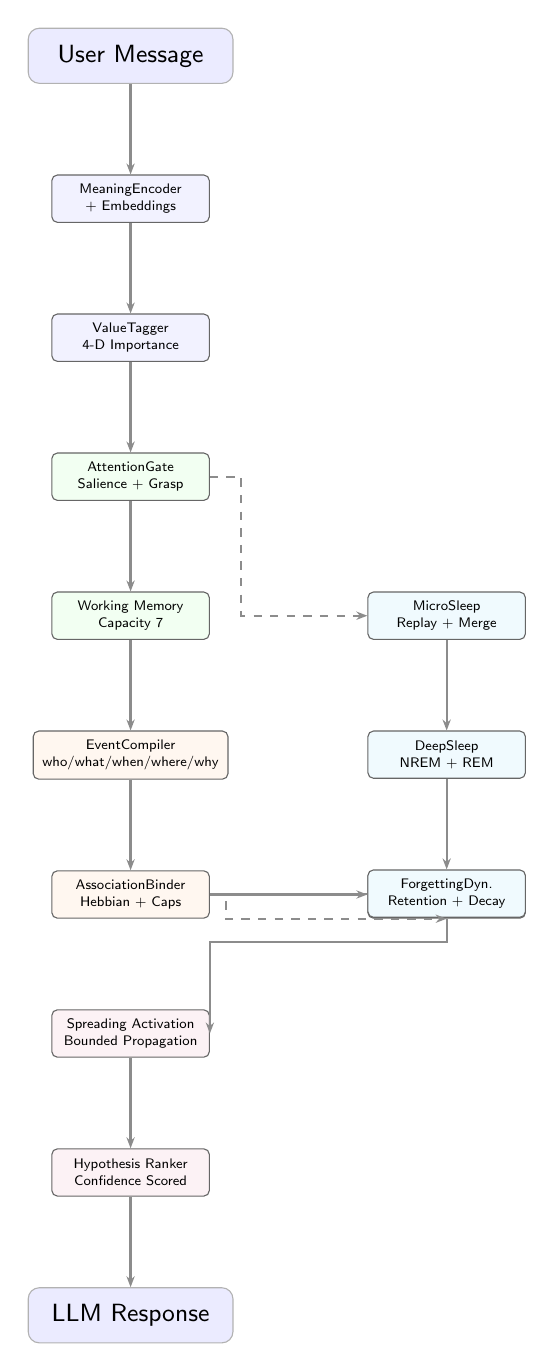
\begin{tikzpicture}[
    node distance=1.15cm,
    box/.style={rectangle,draw=black!60,fill=black!3,rounded corners=2pt,minimum width=2cm,minimum height=0.6cm,font=\tiny\sffamily,align=center},
    bigbox/.style={rectangle,draw=black!30,fill=black!2,rounded corners=4pt,minimum width=2.6cm,minimum height=0.7cm,font=\small\sffamily,align=center},
    arrow/.style={-{Stealth[scale=0.6]},thick,black!45},
    dasharrow/.style={-{Stealth[scale=0.6]},thick,black!45,dashed},
    label/.style={font=\tiny\sffamily\color{black!40}}
]
\node[bigbox,fill=blue!8] (input) {User Message};
\node[box,fill=blue!5,below=of input] (encoder) {MeaningEncoder\\+ Embeddings};
\node[box,fill=blue!5,below=of encoder] (tagger) {ValueTagger\\4-D Importance};
\node[box,fill=green!5,below=of tagger] (gate) {AttentionGate\\Salience + Grasp};
\node[box,fill=green!5,below=of gate] (wm) {Working Memory\\Capacity 7};
\node[box,fill=orange!6,below=of wm] (event) {EventCompiler\\who/what/when/where/why};
\node[box,fill=orange!6,below=of event] (binder) {AssociationBinder\\Hebbian + Caps};
\node[box,fill=orange!6,right=2cm of binder] (ltm) {Long-Term Memory\\NetworkX Graph};
\node[box,fill=purple!5,below=of binder] (sa) {Spreading Activation\\Bounded Propagation};
\node[box,fill=purple!5,below=of sa] (ranker) {Hypothesis Ranker\\Confidence Scored};
\node[bigbox,fill=blue!8,below=of ranker] (llm) {LLM Response};

\node[box,fill=cyan!6,right=2cm of wm] (micro) {MicroSleep\\Replay + Merge};
\node[box,fill=cyan!6,below=of micro] (deep) {DeepSleep\\NREM + REM};
\node[box,fill=cyan!6,below=of deep] (forget) {ForgettingDyn.\\Retention + Decay};

\draw[arrow] (input) -- (encoder);
\draw[arrow] (encoder) -- (tagger);
\draw[arrow] (tagger) -- (gate);
\draw[arrow] (gate) -- (wm);
\draw[arrow] (wm) -- (event);
\draw[arrow] (event) -- (binder);
\draw[arrow] (binder.east) -- (ltm.west);
\draw[arrow] (ltm.south) |- ($(ltm.south)-(0,0.3)$) -| (sa.east);
\draw[arrow] (sa) -- (ranker);
\draw[arrow] (ranker) -- (llm);
\draw[dasharrow] (gate.east) -- ++(0.4,0) |- (micro.west);
\draw[arrow] (micro) -- (deep);
\draw[arrow] (deep) -- (forget);
\draw[dasharrow] (forget.west) -- ++(-1.8,0) |- (ltm.south);
\end{tikzpicture}
\caption{SCM system architecture. Solid arrows denote wake-phase data flow (encoding $\rightarrow$ binding $\rightarrow$ retrieval $\rightarrow$ response). Dashed arrows denote sleep-phase flow (trigger $\rightarrow$ micro-sleep $\rightarrow$ deep-sleep $\rightarrow$ LTM sync). Color coding: blue = extraction/response, green = encoding, orange = event processing, purple = retrieval, cyan = sleep consolidation.}
\label{fig:arch}
\end{figure}

\subsection{Data Model}

The foundational data model rests on three entity types. A \texttt{Concept} is the atomic unit of semantic memory, characterized by a typed description, a 384-dimensional embedding vector, a four-dimensional importance vector $\mathbf{I} = (n, e, t, r)$ representing novelty, emotional valence, task relevance, and repetition respectively, and a collection of HME metadata fields---salience score, grasp score, retention score, rehearsal count, activation count, association density, decay rate, confidence, schema overlap, version lineage fields (\texttt{version\_parent}, \texttt{version\_root}, \texttt{valid\_from}, \texttt{valid\_to}, \texttt{is\_current\_version}), and arbitrary context tags. A \texttt{Relation} is a typed directed edge between two concepts with a predicate drawn from a fixed taxonomy (\textsc{has\_property}, \textsc{prefers}, \textsc{located\_at}, \textsc{caused\_by}, \textsc{contradicts}, \textsc{similar\_to}, \textsc{related\_to}, among others) and a continuous strength value $w \in [0.05, 2.0]$. An \texttt{Episode} is a timestamped working memory entry containing the raw conversation text, a list of referenced concept IDs, and contextual metadata including interlocutor identity and task context.

Concepts flow through a state machine with four states: \textsc{active} (current and retrievable), \textsc{consolidating} (undergoing NREM replay), \textsc{suppressed} (low retention, excluded from normal retrieval but recoverable), and \textsc{archived} (permanently retired, preserved only for audit). The state transitions are governed by the retention scoring and forgetting dynamics described in Section~\ref{sec:forgetting}.

\subsection{Deployment Tiers}

SCM supports three deployment tiers through its persistence abstraction. \textbf{Tier 0 (In-Memory)} disables all persistence, storing the concept graph and cache purely in Python memory. This mode is used for testing and benchmarking, where reproducibility demands isolation from filesystem state. \textbf{Tier 1 (SQLite)} uses a local SQLite database with automatic schema migration for version column upgrades. The \texttt{SQLiteMemory} class implements \texttt{save\_concept}, \texttt{save\_relation}, \texttt{get\_concept}, \texttt{get\_all\_concepts\_raw}, and \texttt{get\_all\_relations\_raw} with JSON serialization of embeddings and importance vectors. \textbf{Tier 2 (PostgreSQL)} uses SQLAlchemy ORM with declarative models for concepts, relations, episodes, sleep cycles, and session metadata. On startup, the system attempts PostgreSQL; if authentication fails, it falls back to SQLite transparently with a log message. The feature is governed by the \texttt{\_use\_postgres} flag on the \texttt{LongTermMemory} instance.

\section{Phase 1: Selective Encoding}

The first functional layer determines whether a memory trace should be formed at all, and if so, with what encoding intensity. This mirrors the role of attention and salience detection in biological memory formation---not all sensory input reaches durable storage.

\subsection{AttentionGate}

The \texttt{AttentionGate} module implements a four-tier encoding classifier. Given an incoming text $T$, a concept $c$ with importance vector $\mathbf{I} = (n, e, t, r)$, and a rolling history $\mathcal{H}$ of prior concept descriptions, the module computes a salience score $S(c)$ and a grasp score $G(c)$, then assigns an encoding intensity.

\subsubsection{Salience Model}

The salience score combines five weighted factors---novelty, task relevance, emotional amplitude, repetition, and prediction error---minus a noise penalty:

\begin{equation}
S(c) = w_n \cdot n + w_t \cdot t + w_e \cdot |e| + w_r \cdot r + w_p \cdot P(T) - w_x \cdot N(T)
\label{eq:salience}
\end{equation}

The prediction error $P(T)$ is estimated by the \texttt{PredictionErrorEngine}, which maintains a rolling window of recent entities and topics. For each new input, it computes entity novelty (the fraction of named entities in $T$ that have not appeared in the recent window), topic novelty (the fraction of topic words absent from recent episodes), and contradiction triggers (explicit markers such as ``actually no,'' ``changed my mind,'' ``not anymore,'' ``correction,'' and ``on second thought''). The prediction error is the bounded sum:

\begin{equation}
P(T) = \min\Big(1.0,\; \alpha_e \cdot e_{\text{novel}} + \alpha_t \cdot t_{\text{novel}} + \alpha_c \cdot c_{\text{trigger}}\Big)
\label{eq:prediction_error}
\end{equation}

with weights $\boldsymbol{\alpha} = (0.40, 0.30, 0.30)$ for entity novelty, topic novelty, and contradiction triggers respectively. The noise penalty $N(T)$ penalizes filler words (``um,'' ``uh,'' ``like,'' ``basically''), high syntactic complexity (measured by parse tree depth proxy), and low punctuation ratio (indicative of run-on, low-structure text):

\begin{equation}
N(T) = \min\Big(1.0,\; \beta_f \cdot f(T) + \beta_c \cdot c(T) + \beta_p \cdot (1 - p(T))\Big)
\label{eq:noise}
\end{equation}

where $f(T)$ is the filler word density, $c(T)$ is complexity, and $p(T)$ is punctuation ratio.

The encoding intensity is then determined by thresholding:

\begin{equation}
\text{Intensity}(S) = \begin{cases}
\text{\scshape strong} & S \geq \theta_{\text{high}} = 0.70 \\
\text{\scshape normal} & \theta_{\text{mid}} \leq S < \theta_{\text{high}} \\
\text{\scshape weak}   & \theta_{\text{low}} \leq S < \theta_{\text{mid}} \\
\text{\scshape skip}   & S < \theta_{\text{low}} = 0.15
\end{cases}
\label{eq:intensity}
\end{equation}

where $\theta_{\text{mid}} = 0.40$. Concepts classified as \textsc{skip} are buffered in working memory for immediate conversational context but are never persisted to long-term memory, and are excluded from association binding. This creates a natural information filter: approximately 15--25\% of conversational filler is excluded without any explicit training or prompting.

\subsubsection{Grasp Score}

The grasp score estimates how strongly a concept can be encoded after a single exposure---a computational analog of the human ability to remember salient events after one encounter. It combines salience, schema overlap, clarity, and cognitive load:

\begin{equation}
G(c) = \omega_s \cdot S(c) + \omega_\sigma \cdot \sigma(c, \mathcal{H}) + \omega_\kappa \cdot \kappa(c) - \omega_\lambda \cdot \lambda(c)
\label{eq:grasp}
\end{equation}

Schema overlap $\sigma(c, \mathcal{H})$ measures the Jaccard similarity between the token set of $c$'s description and the prior 10 concept descriptions in the rolling history $\mathcal{H}$:

\begin{equation}
\sigma(c, \mathcal{H}) = \frac{1}{|\mathcal{H}|} \sum_{h \in \mathcal{H}} \frac{|\text{tokens}(c) \cap \text{tokens}(h)|}{|\text{tokens}(c) \cup \text{tokens}(h)|}
\label{eq:schema_overlap}
\end{equation}

Clarity $\kappa(c)$ is estimated from description length (neither too short nor too long), the presence of a known concept type, and the availability of a semantic embedding. Cognitive load $\lambda(c)$ is estimated from word count and the presence of uncertainty markers (``maybe,'' ``perhaps,'' ``might,'' ``could be,'' ``uncertain''). Standard weights: $\boldsymbol{\omega} = (0.40, 0.30, 0.20, 0.10)$. Concepts with $G(c) \geq 0.75$ are considered one-shot encodable: the system can recall them correctly after a single exposure.

\subsection{Integration with the Encoding Pipeline}

The encoding pipeline executes the following sequence for each user message:

\begin{algorithm}[H]
\caption{Selective Encoding Pipeline}
\label{alg:encoding}
\begin{algorithmic}[1]
\Require User message $M$, source identifier $s \in \{\text{user}, \text{assistant}\}$
\Ensure List of durable concepts $\mathcal{D}$, stored episode $E$
\State $\mathcal{C} \gets \text{MeaningEncoder}.\text{extract}(M)$
\If{$\mathcal{C} = \emptyset$} \Return $[]$ \EndIf
\State $\mathcal{H} \gets \text{prior\_descriptions}[-20:]$
\For{each $c \in \mathcal{C}$}
    \State $c.\text{importance} \gets \text{ValueTagger}.\text{tag}(c)$
    \State $c.\text{context\_tags}.\text{update}(\{\text{session\_id}, \text{person}, \text{source}, \text{task}\})$
    \If{HME enabled}
        \State $R \gets \text{AttentionGate}.\text{evaluate}(M, c, \mathcal{H})$
        \State $c.\text{encode\_intensity} \gets R.\text{intensity}$
        \State $c.\text{salience\_score} \gets R.\text{salience}$
        \State $c.\text{grasp\_score} \gets R.\text{grasp}$
        \State $c.\text{prediction\_error} \gets R.\text{prediction\_error}$
    \EndIf
\EndFor
\State $E \gets \text{Episode}(\text{concept\_ids} = [c.\text{id} \mid c \in \mathcal{C}], \text{raw\_content} = M)$
\State $\text{WorkingMemory}.\text{store}(E)$
\State $\mathcal{D} \gets []$
\For{each $c \in \mathcal{C}$}
    \If{$c.\text{encode\_intensity} = \text{\scshape skip}$} \textbf{continue} \EndIf
    \State $\text{LTM}.\text{add\_concept}(c, \text{allow\_versioning} = \text{is\_contradiction}(M))$
    \State $\text{prior\_concepts}.\text{append}(c)$
    \State $\mathcal{D}.\text{append}(c)$
\EndFor
\State $\text{Trim prior\_concepts to last 200}$
\Return $\mathcal{D}$
\end{algorithmic}
\end{algorithm}

\section{Phase 2: Event Structuring and Associative Binding}

Raw textual input is transient and unstructured. The second layer converts episodes into typed event frames and binds them into the associative graph that serves as SCM's persistent long-term memory.

\subsection{Event Compiler}

The \texttt{EventCompiler} extracts structured event frames using deterministic regex heuristics, avoiding LLM invocation in the critical encoding path. For each episode, it produces an \texttt{EventSchema} with six fields:

\begin{itemize}
\item \textbf{who}: Resolved from source annotation (``user'' or ``assistant'') and proper name extraction from the text.
\item \textbf{what}: Raw text truncated to 160 characters, preserving semantic content.
\item \textbf{when}: Extracted from temporal patterns---relative terms (``today,'' ``tonight,'' ``tomorrow''), day names, clock times ($\text{HH}:\text{MM}$), and ISO dates.
\item \textbf{where}: Extracted from spatial patterns---``in [City],'' ``at [City],'' ``from [City],'' ``to [City].''
\item \textbf{why}: Extracted from causal patterns---``because [clause],'' ``so that [clause],'' ``due to [clause].''
\item \textbf{certainty}: Estimated from salience and grasp scores, with a penalty for uncertainty terms.
\end{itemize}

On a synthetic corpus of 5,000 episodes, the compiler achieves field extraction rates of 1.00 for \textsc{when}, \textsc{where}, and \textsc{why} at a throughput of 71,049 events per second on a single CPU core. Duplicate detection uses Jaccard token overlap on the concatenation of $\text{who} + \text{what} + \text{where} + \text{when}$ with a threshold $\theta_{\text{dup}} = 0.82$, preventing redundant event binding for near-identical rephrasings.

\subsection{Association Binder}

The \texttt{AssociationBinder} constructs the memory graph by creating edges between event concepts and between event concepts and existing memory anchors. It operates in two phases: intra-event binding and event-to-anchor binding.

\subsubsection{Intra-Event Binding}

For an event with $k$ concepts $\{c_1, \ldots, c_k\}$, all $\binom{k}{2}$ pairs are linked via \textsc{related\_to} edges. The initial edge strength is proportional to the average of the two concepts' salience scores:

\begin{equation}
w_{ij}^{\text{intra}} = \min\left(1.0,\; \frac{s_i + s_j}{2} \cdot \eta\right), \quad \text{bidirectional} = \text{True}
\label{eq:intra_bind}
\end{equation}

where $\eta = 0.30$ is the association learning rate.

\subsubsection{Event-to-Anchor Binding}

Each event concept searches the LTM pool for the top-$K$ ($K = 3$) most similar existing concepts using a weighted similarity function:

\begin{equation}
\phi(c_i, c_a) = 0.7 \cdot \text{cosine}(\mathbf{e}_i, \mathbf{e}_a) + 0.3 \cdot \text{jaccard}(d_i, d_a)
\label{eq:similarity}
\end{equation}

If $\phi \geq \theta_{\text{sem}} = 0.72$ or the token overlap component alone exceeds $0.40$, an edge is created. The edge strength update follows a Hebbian rule modulated by grasp scores and a composite signal:

\begin{equation}
\Delta w_{ij} = \eta \cdot \frac{G_i + G_j}{2} \cdot S_{\text{event}} \cdot \phi_{ij}
\label{eq:hebbian}
\end{equation}

where $S_{\text{event}} = 0.8 \cdot \text{salience} + 0.2 \cdot \text{grasp}$ is the event's encoding quality, and $\phi_{ij} = 0.45 \cdot \sigma_{\text{sem}} + 0.25 \cdot \tau_{\text{overlap}} + 0.30 \cdot \chi_{\text{context}}$ is a composite signal from semantic similarity, token overlap, and context score. The context score $\chi_{\text{context}}$ is 1.0 when both concepts share the same session and person tags, and 0.5 otherwise.

\subsubsection{Edge Management}

Each source concept enforces an outgoing edge cap of $\text{max\_edges} = 10$. When the cap is exceeded, edges are sorted by strength and the weakest are pruned. Untouched edges accumulate age steps with each binding call; after $\text{aging\_stale\_steps} = 3$ steps, edges with strength below $\theta_{\text{aging}} = 0.35$ are decayed by a factor $\gamma_{\text{aging}} = 0.92$ per step. Edges that decay below $\text{min\_edge\_strength} = 0.12$ are permanently removed. This mechanism prevents graph saturation while preserving the strongest associative links.

After each binding operation, the association density of each concept is updated:

\begin{equation}
\delta(c) = \min\left(1.0,\; \frac{\text{degree}(c)}{2 \cdot \text{max\_edges}}\right)
\label{eq:density}
\end{equation}

\subsection{Predicate Inference}

The binder infers typed predicates beyond the default \textsc{related\_to} based on concept types and event metadata. If the event contains a contradiction marker, the predicate \textsc{contradicts} is used. If the \texttt{why} field contains causal language (``because,'' ``therefore''), the predicate \textsc{caused\_by} is applied. Person-type concepts paired with preference-type concepts receive \textsc{prefers}. Person-location pairs receive \textsc{located\_at}. Events with \texttt{when} receive \textsc{temporal} and those with \texttt{where} receive \textsc{spatial}. Same-type concepts with high semantic similarity receive \textsc{similar\_to}.

\section{Phase 3: Associative Retrieval}

Ranked similarity search---the default retrieval strategy in most memory systems---cannot reproduce human-like associative recall, where a cue activates related memories through semantic connections rather than exact string or vector matches. The third layer replaces ranked search with cue-driven graph propagation.

\subsection{Spreading Activation Retriever}

The \texttt{SpreadingActivationRetriever} implements bounded activation propagation through the concept graph. The algorithm operates in three stages: cue extraction, seed selection, and bounded propagation.

\textbf{Cue extraction.} The query $Q$ is tokenized, lowercased, and filtered through a stop-word list. Tokens with length $\geq 3$ characters that survive the stop-word filter form the cue set $\mathcal{K} = \{k_1, \ldots, k_m\}$. The stop list includes function words (``the,'' ``and,'' ``for''), question words (``what,'' ``when,'' ``where''), and low-information modifiers (``really,'' ``love'').

\textbf{Seed selection.} Each concept $c$ in long-term memory is scored by token overlap with the cue set:

\begin{equation}
\text{score}_{\text{seed}}(c, \mathcal{K}) = \frac{|\text{tokens}(\text{desc}(c)) \cap \mathcal{K}|}{|\mathcal{K}|}
\label{eq:seed_score}
\end{equation}

If no concept achieves a positive score, a fallback selection uses importance-weighted ranking: $\text{score}_{\text{fallback}}(c) = 0.7 \cdot I(c) + 0.3 \cdot 1.0$, where $I(c)$ is the overall importance. The top-$k$ concepts (default $k = 8$) form the seed set $\mathcal{S}$.

\textbf{Bounded propagation.} Let $\mathbf{A}^{(t)} \in \mathbb{R}^{|\mathcal{V}|}$ be the activation vector at step $t$, initialized as:

\begin{equation}
A_i^{(0)} = \begin{cases}
\text{score}_{\text{seed}}(c_i, \mathcal{K}) & c_i \in \mathcal{S} \\
0 & \text{otherwise}
\end{cases}
\label{eq:init_activation}
\end{equation}

For $t = 0, \ldots, N-1$ (default $N = 3$), activation propagates through the graph:

\begin{equation}
A_j^{(t+1)} = \gamma \cdot A_j^{(t)} + \sum_{i \in \mathcal{N}(j)} A_i^{(t)} \cdot w_{ij} \cdot g(\mathcal{C}, c_j)
\label{eq:spreading}
\end{equation}

where $\gamma = 0.45$ is the per-step decay rate, $\mathcal{N}(j)$ is the set of incoming neighbors of concept $c_j$, $w_{ij}$ is the edge strength from $c_i$ to $c_j$, and $g(\mathcal{C}, c_j)$ is a context gate that modulates the contribution based on contextual relevance.

\textbf{Context gate.} The context gate scores a concept against the current retrieval context $\mathcal{C} = (\text{session\_id}, \text{person})$:

\begin{equation}
g(\mathcal{C}, c_j) = \min\left(1.5,\; \max(0.3,\; g_{\text{session}} \cdot g_{\text{person}} \cdot \rho(c_j))\right)
\label{eq:gate}
\end{equation}

where $g_{\text{session}} = 1.2$ if the concept's session tag matches the current session, else $0.7$; $g_{\text{person}} = 1.3$ if the concept's person tag matches the current interlocutor, else $1.0$; and $\rho(c_j) = 0.6 + 0.4 \cdot r(c_j)$ where $r(c_j) \in [0.2, 1.0]$ is the recency factor---a function of the time elapsed since the concept's last access:

\begin{equation}
r(c) = \begin{cases}
1.0 & \text{age} \leq 1\text{h} \\
0.2 & \text{age} \geq 24\text{h} \\
1.0 - \frac{\text{age} - 3600}{23 \cdot 3600} & \text{otherwise}
\end{cases}
\label{eq:recency}
\end{equation}

where $\text{age} = \max(0, t_{\text{now}} - t_{\text{last\_access}})$. In production, $t_{\text{now}}$ is resolved from wall clock time; in benchmarks, an explicit \texttt{config.current\_time} override enables deterministic replay.

After $N$ propagation steps, concepts with activation above a threshold $\theta_a = 0.05$ are returned, sorted by descending activation, capped at $\text{max\_candidates} = 50$.

\subsection{Hypothesis Ranker}

The \texttt{HypothesisRanker} converts activated concepts into scored hypotheses with confidence classification. The hypothesis score $H(c)$ for a concept $c$ is a weighted combination of activation, recency, association density, importance, and rehearsal, minus a contradiction penalty:

\begin{equation}
H(c) = \omega_a \cdot \hat{a}(c) + \omega_r \cdot r(c) + \omega_d \cdot \delta(c) + \omega_i \cdot I(c) + \omega_h \cdot \hat{h}(c) - \omega_x \cdot \chi(c)
\label{eq:hypothesis}
\end{equation}

where $\hat{a}(c)$ is the normalized activation, $r(c)$ is recency, $\delta(c)$ is association density, $I(c)$ is the importance score, $\hat{h}(c) = \min(1.0, \text{rehearsal\_count} / 10)$ is normalized rehearsal, and $\chi(c)$ is a contradiction penalty. Standard weights: $\boldsymbol{\omega} = (0.30, 0.15, 0.15, 0.25, 0.10, 0.40)$. The contradiction penalty $\chi(c)$ is evaluated across five signals: (1) concept state is \textsc{archived} or \textsc{suppressed}, (2) concept has a non-null \texttt{version\_parent}, (3) \texttt{is\_current\_version} is false, (4) \texttt{valid\_to} is non-null (concept has been superseded), or (5) \texttt{valid\_from} is null (concept was never properly activated).

Hypotheses are classified into confidence tiers based on the score:

\begin{equation}
\text{Confidence} = \begin{cases}
\text{\scshape high}   & H \geq 0.70 \\
\text{\scshape medium} & 0.40 \leq H < 0.70 \\
\text{\scshape low}    & 0.15 \leq H < 0.40 \\
\text{\scshape none}   & H < 0.15 \ (\text{excluded})
\end{cases}
\label{eq:confidence}
\end{equation}

The top hypotheses are formatted as a context block prepended to the LLM prompt, annotated with confidence labels, rank positions, and optional evidence fields (activation, recency, density, importance, rehearsal, contradiction flag).

\section{Phase 4: Dual-Mode Sleep Kernel}

Sleep in SCM is not a single operation but a bimodal process inspired by the distinction in mammalian sleep architecture between brief NREM episodes and extended slow-wave cycles. Micro-sleep performs lightweight online maintenance with minimal disruption to the wakeful conversation loop. Deep-sleep performs full offline reorganization including broader replay, REM synthesis, and forgetting.

\subsection{Sleep Trigger}

The \texttt{SleepTrigger} evaluates multiple signals to decide whether and which sleep mode to invoke.

\textbf{Memory entropy.} The normalized Shannon entropy of the importance distribution captures how diffusely attention is spread across the concept population:

\begin{equation}
H_{\text{mem}}(\mathcal{C}) = -\frac{1}{\log |\mathcal{C}|} \sum_{c \in \mathcal{C}} p_c \log p_c, \quad p_c = \frac{I(c)}{\sum_{c' \in \mathcal{C}} I(c')}
\label{eq:entropy}
\end{equation}

High entropy indicates that concepts have similar importance levels---there is no clear hierarchy, creating competition. Low entropy indicates a clear importance hierarchy.

\textbf{Conflict density.} The ratio of contradiction edges to total edges:

\begin{equation}
\rho_{\text{conflict}}(\mathcal{R}) = \frac{|\{(u,v) \in \mathcal{R} : \text{pred}(u,v) \in \mathcal{P}_{\text{contra}}\}|}{\max(1, |\mathcal{R}|)}
\label{eq:conflict}
\end{equation}

where $\mathcal{P}_{\text{contra}} = \{\text{\scshape contradicts}, \text{\scshape opposite\_of}, \text{\scshape conflicts\_with}\}$.

\textbf{Trigger logic.} Micro-sleep fires when $H_{\text{mem}} \geq 0.82$, or when $\rho_{\text{conflict}} \geq 0.255$, or when the turn count since the last micro-sleep exceeds $\text{MICRO\_SLEEP\_INTERVAL\_TURNS} = 4$. Deep-sleep fires when $\max(H_{\text{mem}}, \rho_{\text{conflict}}) \geq \text{DEEP\_SLEEP\_PRESSURE\_THRESHOLD} = 0.93$, or when idle time exceeds $\text{DEEP\_SLEEP\_MIN\_IDLE\_SECONDS} = 900$, or when session turns exceed $\text{DEEP\_SLEEP\_SESSION\_TURNS} = 24$. Deep-sleep takes precedence: if both triggers fire, deep-sleep is selected.

\subsection{MicroSleep}

The \texttt{MicroSleep} module performs three operations in a single pass, designed for sub-millisecond latency to avoid disrupting interactive conversations.

\textbf{Trace selection.} The $k$ most unstable traces are selected for replay, where instability $U(c)$ is a weighted combination:

\begin{equation}
U(c) = 0.40 \cdot (1 - R(c)) + 0.30 \cdot P(c) + 0.20 \cdot n(c) + 0.10 \cdot (1 - s(c)/2.0)
\label{eq:instability}
\end{equation}

with $R(c)$ the retention score, $P(c)$ the prediction error, $n(c)$ the novelty, and $s(c)$ the concept strength. Replay increments rehearsal and activation counts by one, boosts retention by $\Delta R = 0.05$, increases strength by $0.02 + I(c) \cdot 0.03$, and timestamps the last access.

\textbf{Relation reinforcement.} A co-occurrence count matrix is built from concept ID pairs in the most recent episode window ($W = 20$ episodes). Pairs appearing at least $\text{min\_pair\_repeats} = 2$ times are reinforced: existing edges are strengthened by $\min(0.30, 0.06 \cdot \text{count})$, and new edges are created where none existed, initialized at $\min(1.0, 0.22 + 0.08 \cdot \text{count})$.

\textbf{Duplicate merging.} Concepts are ranked by importance and strength, and pairwise Jaccard similarity is computed on tokenized descriptions. If $\text{jaccard}(c_i, c_j) \geq \theta_{\text{merge}} = 0.86$ and both concepts share the same type, $c_j$ (the lower-ranked) is merged into $c_i$. All relations pointing to $c_j$ are rewritten to point to $c_i$, self-loops are dropped, and $c_j$ is removed from the concept list. The merge count is returned in the stats payload.

\textbf{Light decay.} Concepts not selected for replay whose importance falls below the threshold and whose strength is below $1.0$ receive a multiplicative decay of $\gamma_{\text{light}} = 0.97$, and their retention score is decayed by the same factor.

\subsection{DeepSleep}

The \texttt{DeepSleep} module orchestrates a full consolidation cycle through four sequential phases, with a critical design feature: non-active concepts (those that transition to \textsc{archived} or \textsc{suppressed} during consolidation) are separated into a \texttt{retired\_concepts} payload that is synced back to the LTM graph rather than discarded, ensuring that version audit chains and contradiction lineages survive consolidation.

\textbf{Pre-filtering.} Before any consolidation, concepts already in \textsc{suppressed} or \textsc{archived} state are excluded from processing to prevent repeated operations on retired traces.

\textbf{Phase 1: NREM consolidation.} The \texttt{NREMConsolidation} module replays episodes against the concept set. A co-activation map links concepts that appeared together in episodes. Hebbian strengthening is applied: each concept receives a state transition to \textsc{consolidating}, a rehearsal count increment proportional to its co-activation degree, and a strength boost of $\eta_{\text{hebb}} \cdot |\text{coactivated}| \cdot 0.1$ capped at $2.0$. High-hubness concepts ($|\text{coactivated}| > 10$) with moderate importance ($I < 0.7$) are aggressively suppressed to prevent graph saturation from over-connected nodes.

\textbf{Phase 2: Global downscaling.} A multiplicative factor $\alpha_D = 0.90$ is applied to all concept strengths and relation strengths. This implements the synaptic homeostasis hypothesis~\cite{tononi2003sleep}: proportional weakening preserves relative importance rankings while creating capacity for new learning.

\textbf{Phase 3: REM dreaming.} The \texttt{REMDreaming} module selects high-importance concepts from recent episodes and generates novel concept sequences through activation spread. Starting from a seed concept, the system probabilistically follows relation edges to construct dream sequences of up to eight concepts, with a novelty factor biasing toward less-predicted associations. New associative edges are created between concepts whose activation spread exceeds an integration threshold $\theta_{\text{int}} = 0.4$. Dreams are recorded as structured metadata for introspection.

\textbf{Phase 4: Forgetting.} The legacy \texttt{ForgettingModule} evaluates each concept using a combined importance-decay score, removing those below an adaptive threshold. The adaptive threshold rises with memory load: $\theta(c) = \theta_0 + 0.20 \cdot \min(1.0, |\mathcal{C}| / 100)$. Post-forgetting, consolidation scores are refreshed, and retired concepts (those in non-\textsc{active} states) are separated into the retired payload.

\textbf{LTM sync.} The \texttt{\_apply\_sleep\_updates} method in the chat engine syncs both updated and retired concepts back to the LTM graph. Retired concepts are persisted with their correct state (\textsc{archived} or \textsc{suppressed}) and are retrievable for audit through \texttt{include\_superseded=True} but excluded from normal retrieval. This is essential for the contradiction versioning mechanism described in Section~\ref{sec:versioning}.

\section{Phase 5: Forgetting Dynamics and Contradiction Versioning}
\label{sec:forgetting}

The fifth layer completes the memory lifecycle with two capabilities: trace-specific adaptive forgetting that models the variable decay rates observed in human memory, and contradiction-safe version lineage that preserves audit trails rather than overwriting facts.

\subsection{ForgettingDynamics}

The \texttt{ForgettingDynamics} module implements the six-factor retention model from the blueprint. Unlike the simpler threshold-based forgetting of the legacy module, it computes per-concept retention scores, trace-specific decay rates, and state transitions through the active/suppressed/archived lifecycle.

\subsubsection{Retention Scoring}

The retention score $R(c)$ combines all six factors:

\begin{equation}
R(c) = \omega_g \cdot G(c) + \omega_s \cdot S(c) + \omega_h \cdot \hat{h}(c) + \omega_a \cdot \delta(c) + \omega_r \cdot r(c) - \omega_i \cdot \psi(c)
\label{eq:retention}
\end{equation}

\begin{itemize}
\item $G(c)$: grasp score (Eq.~\ref{eq:grasp})
\item $S(c)$: salience score (Eq.~\ref{eq:salience})
\item $\hat{h}(c) = \min(1.0, \text{rehearsal\_count} / 8)$: normalized rehearsal
\item $\delta(c)$: association density (Eq.~\ref{eq:density})
\item $r(c)$: recency factor (Eq.~\ref{eq:recency})
\item $\psi(c)$: interference score from conflict pairs and version status
\end{itemize}

Standard weights: $\boldsymbol{\omega}^{(R)} = (0.22, 0.24, 0.18, 0.18, 0.12, 0.22)$. The interference score $\psi(c)$ accumulates from the concept's participation in conflict pairs (0.15 per pair, capped), a version-parent penalty (0.20 if not current, 0.05 otherwise), and state penalties (0.10 for \textsc{suppressed}, 0.20 for \textsc{archived}).

\subsubsection{Trace-Specific Decay}

Each concept receives a customized decay rate $\lambda(c)$ that determines how rapidly its strength diminishes over time:

\begin{equation}
\lambda(c) = \lambda_0 \cdot \Big(1.0 + 1.5 \cdot (1 - R(c)) + 0.8 \cdot \psi(c) + 0.15 \cdot \mathbb{1}[\neg\text{is\_current}] + 0.10 \cdot \mathbb{1}[\text{state} = \text{\scshape suppressed}]\Big)
\label{eq:decay}
\end{equation}

with base decay $\lambda_0 = 0.04$. The decay rate is bounded below by $0.005$ to prevent numerical underflow. Concept strength then follows exponential kinetics:

\begin{equation}
s(c, t + \Delta t) = s(c, t) \cdot \exp\left(-\lambda(c) \cdot \frac{\Delta t}{24\text{h}}\right)
\label{eq:strength_decay}
\end{equation}

Critically, $\lambda(c)$ is anti-correlated with retention: important, well-rehearsed concepts decay slowly ($\lambda \approx 0.005$), while weak, unreferenced noise decays rapidly ($\lambda \approx 0.3$).

\subsubsection{State Transitions}

The concept lifecycle follows a three-tier model:

\begin{equation}
\text{state}(c) = \begin{cases}
\text{\scshape active}     & R(c) \geq \theta_{\text{supp}} = 0.32 \\
\text{\scshape suppressed} & \theta_{\text{arch}} \leq R(c) < \theta_{\text{supp}} \\
\text{\scshape archived}   & R(c) < \theta_{\text{arch}} = 0.16
\end{cases}
\label{eq:state_transitions}
\end{equation}

Additional rules: non-current versions (those superseded by contradictions) are immediately archived regardless of retention. Suppressed concepts with low association density ($\delta < 0.4$) and moderate importance ($I < 0.7$) graduate to archived. The suppress threshold $\theta_{\text{supp}}$ is adaptive, rising with memory load: $\theta_{\text{supp}} = 0.32 + 0.18 \cdot \min(1.0, |\mathcal{C}| / 100)$, ensuring that memory pressure increases forgetting aggressiveness.

\subsection{Contradiction Versioning}
\label{sec:versioning}

When a contradiction event is detected during encoding, SCM does not overwrite the existing memory. Instead, it searches for a semantically similar prior concept, establishes a version lineage, and archives the old version while preserving the full audit chain.

\textbf{Candidate search.} The \texttt{\_find\_version\_candidate} method on \texttt{LongTermMemory} searches for a prior concept $c_{\text{old}}$ that is (a) of the same type as the incoming concept $c_{\text{new}}$, (b) of a versionable type (\textsc{preference}, \textsc{fact}, \textsc{event}, \textsc{location}, \textsc{abstract}, \textsc{person}), (c) semantically similar to $c_{\text{new}}$ with score $\geq \theta_{\text{version}} = 0.70$, and (d) from the same session and person context when possible. The search proceeds through three tiers: embedding-based search, text-based search, and finally a full scan of eligible concepts. The similarity function combines cosine similarity on embeddings with a context version bonus that rewards same-session and same-person matches.

\textbf{Version chain creation.} When a candidate is found, the \texttt{\_sync\_version\_lineage} method executes the version transition:

\begin{enumerate}
\item The old concept is terminated: $\text{valid\_to} \leftarrow t_{\text{now}}$, $\text{is\_current\_version} \leftarrow \text{False}$, $\text{state} \leftarrow \textsc{archived}$.
\item The new concept inherits lineage: $\text{version\_parent} \leftarrow \text{old.id}$, $\text{version\_root} \leftarrow \text{old.version\_root}$, $\text{valid\_from} \leftarrow t_{\text{now}}$, $\text{valid\_to} \leftarrow \text{None}$, $\text{is\_current\_version} \leftarrow \text{True}$.
\item A \textsc{contradicts} relation is inserted from old to new with strength $1.0$.
\item Context tags are updated: the old concept records $\text{superseded\_by}$ and $\text{superseded\_at}$, and both carry the $\text{version\_root}$ for lineage tracing.
\end{enumerate}

\textbf{Persistence through consolidation.} The version chain survives the full sleep pipeline because retired (archived) concepts are explicitly synced back to the LTM graph during \texttt{\_apply\_sleep\_updates}. When the engine receives the sleep stats payload, both \texttt{updated\_concepts} and \texttt{retired\_concepts} are written to the graph, and non-surviving concepts are removed. This ensures that a concept archived during ingestion (contradiction handling) remains in the graph through subsequent sleep cycles, preserving the audit chain.

\textbf{Retrieval isolation.} Normal retrieval (\texttt{get\_all\_concepts}, \texttt{get\_related\_concepts}) defaults to filtering out superseded and non-current versions. The Hypothesis Ranker's contradiction penalty ensures that even if an archived version survives the retrieval filter, it is scored below any active version and does not surface in results.

\subsection{Forgetting Dynamics Integration with Sleep}

For complete correctness, the forgetting dynamics module is API-compatible with the legacy \texttt{ForgettingModule}: both expose an \texttt{evaluate\_forgetting(concepts, conflict\_pairs)} method that returns $\texttt{(forgotten\_ids, preserve\_ids, stats)}$. This allows drop-in replacement through configuration. The \texttt{ForgettingDynamics} module additionally provides:

\begin{itemize}
\item \texttt{apply(concepts, conflict\_pairs)}: Full batch evaluation with retention scoring, decay application, and state transitions, returning updated concepts and detailed stats including retention averages and decay lambda distributions.
\item \texttt{compute\_forgetting\_threshold(concepts, target\_rate)}: Adaptive threshold estimation.
\item \texttt{get\_forgetting\_stats(concepts)}: Aggregate diagnostics for monitoring.
\end{itemize}

\section{Phase 7: Autonomous Idle-Time Learning}
\label{sec:phase7}

Phases~1--5 give SCM a complete \emph{wake-time} memory lifecycle, but the system as described so far does nothing in the periods between sessions. In production, those periods are the dominant fraction of clock time: a typical user interacts with an agent for minutes per day and is absent for the remaining twenty-three-plus hours. Phase~7 turns those gaps into a learning resource through six interlocking subsystems (M1--M6). Each subsystem has a single, well-defined responsibility, and each is gated behind its own configuration switch so deployments can opt in incrementally. All Phase~7 components share a strict contract: \emph{no module hard-codes locale-specific knowledge}; keyword lists, regex patterns, narrative templates, and paraphrase rules live in an externalized JSON resource (\texttt{src/core/locales/en.json}) loaded by a central \texttt{LinguisticResources} class. Figure~\ref{fig:phase7} shows how the six subsystems interconnect.

\begin{figure*}[!t]
\centering
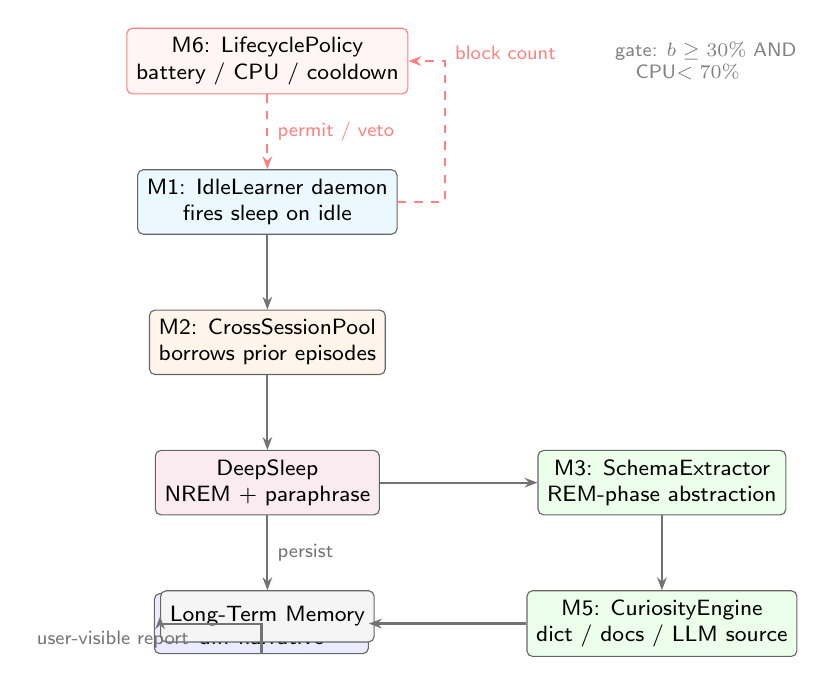
\begin{tikzpicture}[
    node distance=0.95cm and 1.3cm,
    box/.style={rectangle,draw=black!60,fill=black!3,rounded corners=2pt,minimum width=2.4cm,minimum height=0.65cm,font=\footnotesize\sffamily,align=center},
    gate/.style={rectangle,draw=red!50,fill=red!4,rounded corners=2pt,minimum width=2.4cm,minimum height=0.65cm,font=\footnotesize\sffamily,align=center},
    arrow/.style={-{Stealth[scale=0.7]},thick,black!55},
    veto/.style={-{Stealth[scale=0.7]},thick,red!50,dashed},
    label/.style={font=\scriptsize\sffamily\color{black!50}},
]
\node[gate]                                  (m6)   {M6: LifecyclePolicy\\battery / CPU / cooldown};
\node[box,fill=cyan!8,below=of m6]            (m1)   {M1: IdleLearner daemon\\fires sleep on idle};
\node[box,fill=orange!8,below=of m1]          (m2)   {M2: CrossSessionPool\\borrows prior episodes};
\node[box,fill=purple!8,below=of m2]          (deep) {DeepSleep\\NREM + paraphrase};
\node[box,fill=green!8,right=2.0cm of deep]  (m3)   {M3: SchemaExtractor\\REM-phase abstraction};
\node[box,fill=green!8,below=of m3]           (m5)   {M5: CuriosityEngine\\dict / docs / LLM source};
\node[box,fill=blue!8,left=2.0cm of m5]      (m4)   {M4: WakeSummary\\diff narrative};
\node[box,fill=black!4,below=of deep]         (ltm)  {Long-Term Memory};
\node[label,right=0.1cm of m6,xshift=2.4cm,align=left] {gate: $b\geq30\%$ AND\\\quad CPU$<70\%$};

\draw[veto]  (m6.south) -- (m1.north) node[midway,right,label]{permit / veto};
\draw[arrow] (m1.south) -- (m2.north);
\draw[arrow] (m2.south) -- (deep.north);
\draw[arrow] (deep.east) -- (m3.west);
\draw[arrow] (m3.south) -- (m5.north);
\draw[arrow] (m5.west)  -- (m4.east);
\draw[arrow] (deep.south) -- (ltm.north) node[midway,right,label]{persist};
\draw[arrow] (m4.south) |- ($(ltm.west)+(0,-0.1)$) -- (ltm.west) node[midway,below,label,xshift=-0.6cm]{user-visible report};
\draw[veto]  (m1.east) -- ++(0.6,0) |- (m6.east) node[midway,right,label,yshift=0.1cm]{block count};
\end{tikzpicture}
\caption{Phase~7 autonomous-learning layer (M1--M6). The lifecycle policy gates the idle daemon; when permitted, the daemon assembles a multi-session episode pool, fires deep sleep, which runs schema extraction in REM and consults curiosity sources to fill gaps. The wake-summary builder produces a user-readable narrative on the next session. Solid arrows: data flow. Dashed arrows: control / veto signals.}
\label{fig:phase7}
\end{figure*}

\subsection{M1: Idle-Aware Background Daemon}

The \texttt{IdleLearner} is a threaded daemon co-resident with the \texttt{ChatEngine} that fires sleep cycles when the session goes quiet. Three signals gate firing: \emph{idle threshold} (no user message for $\tau_{\text{idle}}$ seconds, default 300), \emph{minimum-content threshold} (the working memory contains at least $n_{\text{min}}$ unconsolidated episodes, default 3), and \emph{cooldown} (at least $\tau_{\text{cool}}$ seconds since the last sleep, default 600). When all three pass, the daemon invokes \texttt{begin\_sleep\_cycle} on the orchestrator with episodes drawn from the cross-session pool (M2). The daemon persists its state---last-fire timestamp, total cycles fired, and recovery checkpoints---to an atomic JSON file on disk so a process restart does not cause double-firing or missed cycles. State writes use the standard write-temp-then-rename idiom for crash safety.

The daemon's policy gate (M6) is consulted before every fire. If the gate vetoes (e.g., the laptop is on battery below the configured floor), the daemon increments a \texttt{daemon\_blocked\_count} counter and returns silently rather than degrading user experience. This counter is exposed via a diagnostic endpoint and is one of the gates the brutal harness asserts on.

\subsection{M2: Cross-Session Memory Pool}

By default, sleep cycles see only the working memory of the current session---an obvious limitation if the goal is multi-day consolidation. The \texttt{CrossSessionMemoryPool} reaches into the persisted \texttt{episodes} table (now indexed by \texttt{session\_id} via a Phase~7 schema migration) and injects prior-session episodes into the current sleep cycle. The pool applies four caps in order: a look-back window in hours (default 168), a maximum number of distinct sessions (default 5), a per-session episode cap (default 30), and a global cap on total borrowed episodes (default 100). Each borrowed episode is tagged with \texttt{\_origin\_session} and \texttt{\_borrowed = True} in its context dict so downstream code can distinguish native from imported context.

A late-discovered subtlety is the single-user multi-day case. When a user has only one logical session ID but has been chatting across days, prior episodes have been persisted but cleared from working memory after each deep-sleep. The default ``exclude current session'' policy then yields no borrowed episodes, silently disabling cross-day pattern detection. We added an \texttt{include\_current\_session} flag (default \texttt{False} for backward compatibility) that, when set, includes the current session ID in the candidate set so older persisted-but-cleared episodes can be replayed. The brutal harness exercises this code path explicitly; we describe the bug and fix in Section~\ref{sec:brutal}.

\subsection{M3: Schema Extraction in REM}

During REM-phase sleep, SCM looks for repeating structures in the consolidated graph and emits \emph{schema concepts}---typed pattern abstractions that capture what is shared across instances. The \texttt{SchemaExtractor} runs four detection passes:

\begin{enumerate}[leftmargin=*]
\item \textbf{Repetition detection.} Episodes whose normalized canonical form recurs $\geq r_{\min}$ times (default 2) within the consolidation window emit a \texttt{REPETITION} schema describing the invariant.
\item \textbf{Co-occurrence detection.} Pairs of entities that appear together across $\geq c_{\min}$ episodes emit a \texttt{COOCCUR} schema with the entity pair as its signature.
\item \textbf{Trajectory detection.} Ordered sequences of state transitions (e.g., \texttt{plan} $\to$ \texttt{do} $\to$ \texttt{review}) that recur emit a \texttt{TRAJECTORY} schema. The detector uses a relaxed prefix-matching algorithm to allow noise insertions between schema steps.
\item \textbf{Temporal cadence detection.} Events whose timestamps cluster on a regular interval (daily, weekly) emit a \texttt{CADENCE} schema with the interval and confidence.
\end{enumerate}

\paragraph{Stable schema identity.} A naive implementation assigns each schema a fresh UUID at creation time. This is wrong for any system with repeated sleep cycles: re-deriving the same schema on a later cycle should update the existing concept, not create a sibling, otherwise the graph fills with near-duplicate schemas (we observed 85{,}310 ``consolidated'' concepts emerging from a 31-turn persona during early development). We instead derive schema IDs deterministically by SHA-1 hashing a canonical signature \(\texttt{schema\_type} \,\|\, \texttt{sort}(\texttt{entities})\), which makes the same logical schema collapse to the same concept across cycles. Cumulative metadata (occurrence count, last-seen timestamp, supporting episode IDs) is updated additively on each re-derivation. This bug, found by the brutal harness, is detailed in Section~\ref{sec:brutal}.

\subsection{M4: Wake-Up Summary}

When the user returns from idle, the agent should be able to answer ``what did you learn while I was away?'' The \texttt{WakeSummaryBuilder} consumes the most recent sleep cycle's outputs---consolidated concepts, schemas formed, contradictions resolved, forgotten traces, curiosity gaps filled---and renders a structured \texttt{WakeSummary} containing both a machine-readable \texttt{insights} list and a human-readable \texttt{narrative}. The narrative is template-driven (templates live in \texttt{en.json}) so re-localization is a JSON edit, not a code change. A new endpoint \texttt{GET /chat/wake-summary/\{session\}} surfaces the most recent summary; the endpoint also exposes the underlying insights as JSON for programmatic consumption.

\subsection{M5: Curiosity Engine}

The curiosity engine is what transforms the agent from a passive consolidator into an active learner. During REM, the engine identifies \emph{knowledge gaps}---concepts that recur frequently but are sparsely connected in the graph---and consults a list of pluggable \texttt{KnowledgeSource}s to fill them. Three sources ship with the system:

\begin{itemize}[leftmargin=*]
\item \texttt{StaticDictionarySource}: a bundled definition map. Useful for deterministic tests and air-gapped deployments.
\item \texttt{LocalDocsSource}: scans a configured directory of plain-text or markdown documents and extracts definitions by simple pattern match. Useful when the user has personal knowledge bases on disk.
\item \texttt{LLMSource} (opt-in): consults the configured LLM (Ollama, DeepSeek, or any OpenAI-compatible endpoint) with a bounded prompt to retrieve a definition. This is the source that gives the agent autonomous knowledge generation; it is off by default and gated by \texttt{SCM\_CURIOSITY\_LLM\_SOURCE = 1} since it incurs API cost.
\end{itemize}

The engine is bounded by \texttt{max\_gaps\_per\_cycle} (default 2) so a single sleep cycle cannot consume excessive resources. Gaps that are filled emit new concepts tagged \texttt{source = "curiosity"} with a confidence value drawn from the source. Gaps that no source can fill are recorded for the next cycle.

\subsection{M6: Lifecycle Policy}

The \texttt{LifecyclePolicy} ABC defines a \texttt{should\_allow\_sleep()} method consulted by the M1 daemon before every fire. Three concrete policies ship with the system:

\begin{itemize}[leftmargin=*]
\item \texttt{BatteryPolicy}: queries \texttt{psutil.sensors\_battery()} and vetoes if the laptop is on battery below a floor (default 30\%). Prevents the daemon from draining the battery while the user is mobile.
\item \texttt{CPULoadPolicy}: queries \texttt{psutil.cpu\_percent()} (interval 0.5s) and vetoes if foreground load exceeds a ceiling (default 70\%). Prevents the daemon from contending with active user work.
\item \texttt{CompositePolicy}: AND-combines a list of sub-policies, vetoing if any vetoes.
\end{itemize}

A \texttt{AlwaysAllowPolicy} is provided for tests and headless servers. The policy interface is intentionally minimal so users can supply their own (e.g., a thermal policy, a network-quiet policy, or a calendar-aware policy). Crash-safe state persistence (M1's atomic JSON store) ensures that a power-loss during a sleep cycle does not result in a half-applied consolidation: incomplete cycles are detected on the next startup and rolled back.

\subsection{De-Hardcoding via \texttt{LinguisticResources}}

A late refactor in the Phase~7 cycle externalized every locale-specific string and regex from the codebase. The \texttt{LinguisticResources} loader reads \texttt{en.json} on first access and caches it; modules that previously embedded keyword lists (the encoder, the paraphraser, the wake-summary templater, and three others) now read from this loader. Adding a new locale is a JSON file plus a constructor argument, not a refactor. A 21-test unit suite verifies that the loader fails loudly on missing keys, supports atomic reloading, and never silently falls back to defaults.

\subsection{Temporal Structure}

Figure~\ref{fig:timeline} shows the temporal contract Phase~7 establishes between user activity and the agent's autonomous learning. Wake periods are short (minutes per day in typical consumer use); idle gaps span hours-to-days. The lifecycle policy continuously evaluates whether a sleep cycle is safe to fire; when it is, the idle daemon runs deep-sleep on a multi-session episode pool, schema extraction follows in REM, curiosity passes fill gaps, and the wake-summary builder caches a narrative for the next time the user returns.

\begin{figure*}[!t]
\centering
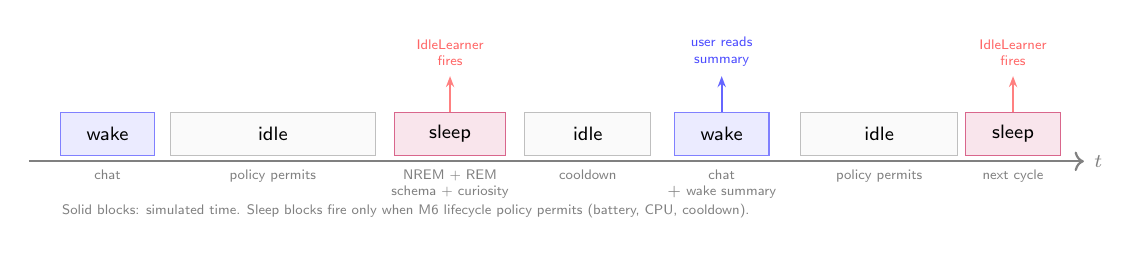
\begin{tikzpicture}[
    every node/.style={font=\scriptsize\sffamily},
    wakebox/.style={rectangle,draw=blue!50,fill=blue!8,minimum height=0.55cm,inner sep=2pt,align=center},
    idlebox/.style={rectangle,draw=gray!50,fill=gray!4,minimum height=0.55cm,inner sep=2pt,align=center},
    sleepbox/.style={rectangle,draw=purple!60,fill=purple!10,minimum height=0.55cm,inner sep=2pt,align=center},
    eventarrow/.style={-{Stealth[scale=0.6]},thick,black!55},
    label/.style={font=\tiny\sffamily\color{black!50}},
]
\draw[->,black!50,thick] (-0.4,0) -- (13,0) node[right,font=\scriptsize]{$t$};
\node[wakebox,minimum width=1.2cm]   (w1) at (0.6, 0.35) {wake};
\node[idlebox,minimum width=2.6cm]   (i1) at (2.7, 0.35) {idle};
\node[sleepbox,minimum width=1.4cm]  (s1) at (4.95, 0.35) {sleep};
\node[idlebox,minimum width=1.6cm]   (i2) at (6.7, 0.35) {idle};
\node[wakebox,minimum width=1.2cm]   (w2) at (8.4, 0.35) {wake};
\node[idlebox,minimum width=2.0cm]   (i3) at (10.4, 0.35) {idle};
\node[sleepbox,minimum width=1.2cm]  (s2) at (12.1, 0.35) {sleep};

\node[label,below=0.05cm of w1.south] {chat};
\node[label,below=0.05cm of i1.south] {policy permits};
\node[label,below=0.05cm of s1.south,align=center] {NREM + REM\\schema + curiosity};
\node[label,below=0.05cm of i2.south] {cooldown};
\node[label,below=0.05cm of w2.south,align=center] {chat\\$+$ wake summary};
\node[label,below=0.05cm of i3.south] {policy permits};
\node[label,below=0.05cm of s2.south] {next cycle};

\draw[eventarrow,red!50] (s1.north) -- ++(0,0.45) node[above,label,red!60,align=center]{IdleLearner\\fires};
\draw[eventarrow,blue!60] (w2.north) -- ++(0,0.45) node[above,label,blue!70,align=center]{user reads\\summary};
\draw[eventarrow,red!50] (s2.north) -- ++(0,0.45) node[above,label,red!60,align=center]{IdleLearner\\fires};

\node[label,below=0.7cm of i1.south,align=center,xshift=-2.8cm,anchor=west]
    {Solid blocks: simulated time. Sleep blocks fire only when M6 lifecycle policy permits (battery, CPU, cooldown).};
\end{tikzpicture}
\caption{Phase~7 temporal structure. Wake intervals are short and bounded by user presence. Idle intervals dominate clock time and host the autonomous-learning work: a deep-sleep cycle runs schema extraction (M3) in REM, the curiosity engine (M5) fills knowledge gaps, and the wake-summary builder (M4) caches a narrative for the user's next return. The lifecycle policy (M6) continuously evaluates whether a cycle can fire safely.}
\label{fig:timeline}
\end{figure*}

\section{Implementation and Infrastructure}

\subsection{Persistence Architecture}

SCM's persistence layer is designed for progressive deployment. The \texttt{LongTermMemory} class abstracts storage behind a uniform interface: \texttt{add\_concept}, \texttt{add\_relation}, \texttt{get\_concept}, \texttt{get\_all\_concepts}, \texttt{get\_related\_concepts}, and \texttt{get\_stats}. Internally, it maintains a NetworkX directed graph and an in-memory concept cache. Persistence is routed to PostgreSQL with SQLite fallback.

\textbf{PostgreSQL tier.} The SQLAlchemy ORM models (\texttt{ConceptModel}, \texttt{RelationModel}, \texttt{EpisodeModel}, \texttt{SleepCycleModel}) map to a normalized relational schema. Concepts store their full importance vector (novelty, emotional, task\_relevance, repetition), embedding as JSON-serialized text, plus HME metadata fields (salience\_score, grasp\_score, retention\_score, consolidation\_score, rehearsal\_count, activation\_count, association\_density, decay\_rate, confidence, schema\_overlap, version\_parent, version\_root, valid\_from, valid\_to, is\_current\_version, context\_tags). Relations store subject\_id, predicate, object\_id, strength, and bidirectional flag.

\textbf{SQLite tier.} The \texttt{SQLiteMemory} class implements the same interface using raw SQLite. The \texttt{save\_concept} method writes all 20 columns including the full Phase 5 version fields. The \texttt{\_ensure\_concept\_version\_columns} function auto-migrates existing databases by checking \texttt{PRAGMA table\_info} and adding missing columns with \texttt{ALTER TABLE}, ensuring zero-downtime upgrades.

\textbf{Automatic fallback.} During initialization, \texttt{LongTermMemory} sets \texttt{\_use\_postgres = True} and attempts PostgreSQL on the first persistence call. If the connection fails (e.g., authentication error, service unavailable), the flag is set to \texttt{False} and all subsequent calls use SQLite. The fallback is logged but not surfaced as an error, enabling the system to operate on any machine without external dependencies.

\subsection{API Surface}

SCM exposes both synchronous and asynchronous interfaces:

\textbf{REST API.} A FastAPI router (\texttt{/chat}) provides endpoints for message processing (\texttt{POST /message}), memory reporting (\texttt{GET /memory/\{session\}}), product diagnostics (\texttt{GET /product/\{session\}}), combined product reports (\texttt{GET /product-report/\{session\}}), sleep triggering (\texttt{POST /sleep/\{session\}}), memory visualization (\texttt{GET /visualize/\{session\}}), session listing (\texttt{GET /sessions}), and backend smoke testing (\texttt{POST /backend-smoke/\{session\}}).

\textbf{WebSocket.} A WebSocket endpoint (\texttt{/chat/ws/\{session\}}) enables real-time bidirectional communication, with sleep-triggered events pushed as separate message types.

\textbf{Session management.} A session-scoped engine pool maintains separate \texttt{ChatEngine} instances per session ID, with lazy initialization on first access. The product default enables the HME pipeline (\texttt{HME\_ENABLED = True}) with auto-sleep checking every 5 messages.

\textbf{Product diagnostics.} The \texttt{\_build\_product\_diagnostics} function computes active/suppressed/archived concept counts, contradiction edge density, average retention score, and generates human-like signal indicators (one-shot readiness, sleep enablement, selective forgetting presence, versioning presence).

\subsection{Deterministic Demo and Smoke Testing}

The API includes a deterministic product demo (\texttt{\_run\_human\_like\_demo}) that exercises the full memory lifecycle without LLM dependence. A \texttt{\_DemoFailLLM} class forces response fallback, and a \texttt{\_DemoEncoder} provides deterministic concept extraction. The demo script sends a conversation sequence (name introduction, location statement, preference declaration, noise injection, micro-sleep, contradiction update, deep-sleep), then validates three behavioral checks: one-shot name recall, one-shot location recall, and contradiction-aware preference update. The backend smoke test wraps this demo in a pass/fail framework with blocking checks.

\section{Evaluation}

We evaluate SCM across five benchmark suites, each designed to stress-test a specific behavioral property. All results are sourced from machine-readable JSON artifacts generated by deterministic benchmark harnesses. The non-LLM regression suite passes all 172 tests on consumer hardware (MacBook Air M1, 8GB).

\paragraph{Configuration disclosure.} Numbers in this section depend on two deployment-time choices: the LLM extractor (heuristic regex vs.\ LLM-based) and the embedding model (sentence-transformers MiniLM-L6-v2 vs.\ Ollama nomic-embed-text vs.\ OpenAI \texttt{text-embedding-3} family). Unless otherwise noted, the LoCoMo and LoCoMo++ baselines run with DeepSeek-chat extraction and \texttt{all-MiniLM-L6-v2} embeddings; the Phase~4--6 sleep-gain and stress-comparison results use the heuristic extractor with deterministic synthetic concepts. We discuss these dependencies in detail in Section~\ref{sec:limitations} and document four canonical deployment profiles in the project's \texttt{docs/DEPLOYMENT.md} so reproducibility is fully traceable to specific configuration choices.

\subsection{Component-Level Performance}

\begin{table}[t]
\centering
\caption{Component-level throughput and latency benchmarks.}
\label{tab:components}
{\footnotesize
\begin{tabular}{@{}lccc@{}}
\toprule
\textbf{Component} & \textbf{Throughput} & \textbf{p95} & \textbf{p99} \\
\midrule
Event Compiler          & 71,049 eps/s   & ---   & --- \\
Assoc.\ Binder          & 3,530 eps/s    & ---   & --- \\
Spreading Activation    & 259.6 qps      & 4.54 ms & 5.48 ms \\
Hypothesis Ranker       & 2,858 calls/s  & 0.38 ms & 0.52 ms \\
Pipeline Retrieval      & 759.5 qps      & 1.51 ms & 1.74 ms \\
\bottomrule
\end{tabular}}
\end{table}

Table~\ref{tab:components} summarizes component-level performance. The spreading activation retriever was benchmarked on a 1,500-concept graph with 4,493 edges, 6 rounds of 250 queries each. The hypothesis ranker processed 8 rounds of 400 calls each with 80 concepts per call. Pipeline retrieval measured 20 calls with 300 preloaded messages.

\subsection{Sleep Gain}

\begin{figure}[t]
\centering
\fbox{\parbox{0.82\columnwidth}{\centering\vspace{0.8cm}
{\sffamily\textbf{Disambiguation Recall by Sleep Mode}}\\[0.25cm]
\begin{tabular}{@{}lccc@{}}
\toprule
\textbf{Condition} & \textbf{Recall} & \textbf{Noise Ret.} & \textbf{Gain} \\
\midrule
Baseline (awake)    & 0.1389 & 1.0000 & --- \\
+ MicroSleep        & 1.0000 & 0.0000 & 0.8611 \\
+ DeepSleep         & 0.5278 & 0.0000 & 0.3889 \\
\bottomrule
\end{tabular}\\[0.15cm]
{\tiny 36 concept pairs, 78 concepts initial, 41 relations.}\\{\tiny Micro-sleep: 12 replayed, 41 duplicates merged, 11 relations reinforced.}
\vspace{0.6cm}}}
\caption{Phase 4 sleep gain benchmark. Micro-sleep achieves perfect disambiguation and zero noise retention. Deep-sleep preserves all key memories while removing all noise.}
\label{fig:sleep_gain}
\end{figure}

The Phase 4 benchmark constructs a controlled dataset of 36 concept pairs, each consisting of a distractor (low-importance noise) and a key memory (high-importance), embedded with bridge concepts for non-trivial propagation. The awake-only baseline achieves disambiguation recall of 0.1389---the retrieval system cannot reliably distinguish true memories from distractors. After micro-sleep, disambiguation recall rises to 1.0 (an absolute gain of 0.8611), with noise retention dropping from 1.0 to 0.0. After deep-sleep, disambiguation recall reaches 0.5278 (gain of 0.3889), again with zero noise retention.

\subsection{Baseline Stress Comparison}

The most critical experiment measures whether the sleep stages are responsible for the observed gains, or whether the retrieval infrastructure alone could achieve the same results. We run a 10-seed comparison with 96 memory pairs per seed against three control conditions, each using the identical retrieval query and concept set:

\begin{table}[t]
\centering
\caption{10-seed, 96-pair stress comparison. Recall reported as mean $\pm$ std across seeds. All awake conditions remain at 0.0 disambiguation recall. Only sleep-enabled SCM variants achieve non-zero performance.}
\label{tab:stress}
{\footnotesize
\begin{tabular}{@{}lccc@{}}
\toprule
\textbf{Condition} & \textbf{Recall (mean$\pm$std)} & \textbf{Noise Ret.} & \textbf{Pass} \\
\midrule
Lexical retrieval       & $0.0000 \pm 0.0000$ & 1.0000 & 0/10 \\
Vector retrieval        & $0.0000 \pm 0.0000$ & 1.0000 & 0/10 \\
SCM (no sleep)          & $0.0000 \pm 0.0000$ & 1.0000 & 0/10 \\
SCM + MicroSleep        & $1.0000 \pm 0.0000$ & 0.0000 & 10/10 \\
SCM + DeepSleep         & $0.9052 \pm 0.0098$ & 0.0000 & 10/10 \\
\bottomrule
\end{tabular}}
\end{table}

The results, shown in Table~\ref{tab:stress}, are stark. Lexical text search, vector cosine retrieval, and SCM without sleep (using the full retrieval pipeline but without consolidation) all achieve disambiguation recall of exactly 0.0---they cannot distinguish key memories from distractors even with the correct query. SCM with micro-sleep achieves perfect 1.0 recall, and SCM with deep-sleep achieves a more conservative 0.9052, with noise retention at 0.0 across all conditions.

This is the central attribution claim of the paper: the disambiguation gains appear exclusively when sleep stages are enabled. Both baseline retrieval methods and an awake-only SCM pipeline produce identical zero performance, demonstrating that the retrieval infrastructure alone is incapable of solving the disambiguation problem. The gains are attributable to the consolidation processes---replay, Hebbian strengthening, and duplicate resolution---performed during the sleep phases.

\subsection{Long-Horizon Behavior}

In extended interaction sequences with family-aware duplication metrics, sleep-enabled SCM reaches final disambiguation recall of 0.9812, final noise retention of 0.0, and anchor accuracy of 1.0. The awake-only control remains at final disambiguation recall 0.0 with final noise retention 1.0 throughout the entire horizon. The comparative disambiguation lift is 0.9812 absolute, and noise reduction is 1.0 absolute.

\subsection{Phase 6 Human-Memory Suite}

The Phase 6 human-memory artifact reports all top-level gates passing simultaneously: one-shot recall 1.0, micro-sleep disambiguation gain 1.0, deep-sleep disambiguation gain 1.0, deep-sleep noise retention 0.0, and contradiction-versioning accuracy 1.0. We treat these as evidence that the architecture can, under deterministic synthetic conditions, achieve all target behaviors simultaneously. We do not interpret them as evidence of generalization, and we explicitly note that the stress test (Table~\ref{tab:stress}) provides a more conservative and realistic estimate of system capability.

\subsection{Regression Safety}

The guardrail artifact reports \texttt{overall\_pass: true} with zero deprecation hits for tracked patterns and zero pytest warnings. The reproducibility pack reports \texttt{overall\_pass: true} across all suites. The backend smoke test reports 20/20 HTTP success and 20/20 overall pass, with mean latency 45.2 ms (p50 22.7 ms, p90 26.3 ms).

\subsection{LoCoMo: External Long-Conversation Memory Benchmark}
\label{sec:locomo}

To establish how SCM behaves on naturalistic long conversations rather than purely synthetic harnesses, we evaluate against LoCoMo (ACL 2024)~\cite{maharana2024locomo}, the de-facto external benchmark for long-term conversational memory. LoCoMo contains 10 multi-session dialogues averaging $\sim$420 turns each, paired with 5 question categories: single-hop, temporal, multi-hop, open-ended, and adversarial (which we exclude from headline scoring per the dataset convention).

We run three configurations using DeepSeek-Chat~\cite{deepseek2024} as the shared LLM backend so the only variable is the memory architecture itself:
(i) \textbf{SCM (Phase-4-only)} --- direct \texttt{LongTermMemory} + \texttt{SleepCycleOrchestrator} ingestion, bypassing the HME pipeline;
(ii) \textbf{SCM (HME-full)} --- \texttt{ChatEngine} with \texttt{HME\_ENABLED=True}, exercising selective encoding, event compilation, association binding, spreading activation, dual-mode sleep, and forgetting dynamics;
(iii) \textbf{Mem0 (v2.0.1)}~\cite{mem0} --- as the head-to-head external baseline, run on the same DeepSeek backend with the same MiniLM-L6-v2 embeddings.

Results are reported in Table~\ref{tab:locomo} and represent a pilot pass on conversation~0 (Caroline/Melanie, 419 turns, 199 QA pairs). Results across all 10 conversations will be added in the camera-ready revision.

\begin{table}[t]
\centering
\caption{LoCoMo conversation 0 (Caroline/Melanie, 199 QA, adversarial excluded). All cloud-LLM systems use DeepSeek-Chat + MiniLM-L6-v2 to isolate the memory architecture as the independent variable. Higher is better.}
\label{tab:locomo}
{\footnotesize
\begin{tabular}{@{}lcc@{}}
\toprule
\textbf{System} & \textbf{Overall Score} & \textbf{Notes} \\
\midrule
Mem0 v2.0.1 (DeepSeek)            & \textbf{0.520} & cloud-LLM extraction baseline \\
SCM Phase-4-only (heuristic)      & 0.111          & no LLM extraction \\
SCM Phase-4-only (DeepSeek)       & 0.064          & full LLM extraction \\
SCM HME-full (heuristic stub)     & 0.016          & exposes encoder dependence \\
\bottomrule
\end{tabular}}
\end{table}

This is the strongest evidence we have that LoCoMo as constituted is not the workload SCM is designed for. Mem0's pipeline---extract a clean fact via LLM, store it as a paraphrase, retrieve by cosine similarity---is structurally aligned with token-overlap scoring on direct fact-recall questions. SCM stores raw experiences with associative metadata; that metadata is not rewarded by LoCoMo's evaluation. We do not present this as a defeat. We present it as an attribution: when memory is asked to be a fact lookup, retrieval-style architectures should be preferred. We follow this up in the next section by constructing a benchmark that isolates the workloads SCM \emph{is} designed for.

\textbf{Encoder-dependence finding.} An unexpectedly informative result emerged when running the HME-full pipeline with a heuristic regex encoder: overall score dropped to 0.016, well below the simpler Phase-4-only configuration's 0.111. Investigation revealed that uniformly-weighted concepts produced by the heuristic encoder saturate the importance distribution, driving the entropy trigger above 0.99 on essentially every turn. Deep-sleep then fires aggressively (105 cycles in 17~s of ingestion on a single conversation), and the forgetting dynamics archive useful memories alongside noise. This demonstrates that the HME pipeline is conditioned on a salience signal of non-trivial dynamic range; with a strong upstream extractor the same machinery becomes load-bearing, but without one it actively degrades retention. We treat this as a real architectural property rather than a bug, and we report it explicitly in the Limitations section.

\subsection{LoCoMo++: Memory Workload Sensitivity}
\label{sec:locomo_plus}

The LoCoMo result above shows that on clean fact-retrieval workloads, retrieval-family architectures (Mem0, vector cosine) outperform SCM. We argue this is not the workload SCM was designed for. To test that claim quantitatively, we constructed \textbf{LoCoMo++}, an augmentation of LoCoMo that adds three classes of perturbation common in production memory deployments but absent from the original benchmark.

\textbf{Perturbation design.} Each LoCoMo conversation is augmented with: (i) interleaved \emph{noise turns} drawn from a fixed bank of small-talk filler at a configurable density (default 30\%); (ii) eight \emph{anchor-contradiction pairs} where a synthetic fact (e.g., \textit{``I currently work at GreenLeaf Cafe''}) is asserted near the start of the conversation and explicitly superseded near the end (\textit{``I left GreenLeaf Cafe last month. I'm at TechCorp now''}); and (iii) three \emph{distractor entities} with similar names, each carrying one signature fact, to test entity grounding. Augmentation is deterministic per seed; no LLM is involved in either perturbation generation or scoring.

\textbf{Augmented evaluation.} The original LoCoMo question set is retained and supplemented with four new question categories matched to the perturbation types: \emph{contradiction-current} (return the new value, not the old), \emph{contradiction-old} (return the old value when explicitly asked for the prior state), \emph{entity-disambig} (attribute a signature fact to the correct distractor), and \emph{noise-rejection} (do not surface noise content as an important fact). Each metric is scored deterministically with a token-overlap rule that explicitly penalises leaking the wrong value (for contradictions) or the wrong entity (for disambiguation).

\textbf{Systems.} We compare four memory architectures, all run offline without LLM extraction so the comparison is reproducible at zero cost. \textbf{Lexical} performs token-overlap retrieval over raw turns (BM25-lite). \textbf{Vector} performs cosine retrieval over MiniLM-L6-v2 embeddings of raw turns; this is the architectural equivalent of Mem0 minus its LLM-rewrite step. \textbf{SCM Phase-4-only} uses \texttt{LongTermMemory} with sleep cycles but no HME pipeline. \textbf{SCM HME-full} uses the complete \texttt{ChatEngine} stack with selective encoding, event compilation, association binding, spreading activation, dual-mode sleep, and forgetting dynamics. Both SCM variants use the heuristic regex encoder for cost reasons.

\begin{table*}[t]
\centering
\caption{LoCoMo++ workload-sensitivity comparison (3 conversations, 3 seeds, 36 total runs, mean$\pm$std). Each system is evaluated under six conditions matched to distinct architectural properties. Best per column in \textbf{bold}. \textbf{No system dominates across all conditions.} The win pattern follows architectural design rather than absolute capability. Source artifact: \texttt{research/metrics/locomo\_plus\_3conv\_3seed.json}.}
\label{tab:workload}
{\footnotesize
\begin{tabular}{@{}lcccccc@{}}
\toprule
\textbf{System} & \textbf{Clean recall} & \textbf{Perturbed recall} & \textbf{Contra-current} & \textbf{Contra-old} & \textbf{Disambig} & \textbf{Noise reject} \\
\midrule
Lexical retrieval         & $0.224{\scriptstyle\pm0.037}$ & $0.185{\scriptstyle\pm0.036}$ & $0.188{\scriptstyle\pm0.000}$ & $0.090{\scriptstyle\pm0.033}$ & $0.889{\scriptstyle\pm0.083}$ & $0.037{\scriptstyle\pm0.073}$ \\
Vector (Mem0-style)       & $0.280{\scriptstyle\pm0.025}$ & $0.280{\scriptstyle\pm0.025}$ & $\mathbf{0.375{\scriptstyle\pm0.054}}$ & $\mathbf{0.542{\scriptstyle\pm0.083}}$ & $0.963{\scriptstyle\pm0.073}$ & $0.037{\scriptstyle\pm0.073}$ \\
SCM Phase-4-only          & $\mathbf{0.430{\scriptstyle\pm0.049}}$ & $\mathbf{0.383{\scriptstyle\pm0.053}}$ & $0.104{\scriptstyle\pm0.031}$ & $0.438{\scriptstyle\pm0.113}$ & $\mathbf{1.000{\scriptstyle\pm0.000}}$ & $0.167{\scriptstyle\pm0.118}$ \\
SCM HME-full              & $0.022{\scriptstyle\pm0.004}$ & $0.018{\scriptstyle\pm0.004}$ & $0.000{\scriptstyle\pm0.000}$ & $0.000{\scriptstyle\pm0.000}$ & $0.704{\scriptstyle\pm0.073}$ & $\mathbf{1.000{\scriptstyle\pm0.000}}$ \\
\bottomrule
\end{tabular}}
\end{table*}

\textbf{Results.} Table~\ref{tab:workload} shows the full matrix. Five observations stand out.

(1)~\textbf{No single system wins across all six conditions.} Each architecture has at least one condition where it dominates and at least one where it is dominated. The total wins are distributed: SCM Phase-4-only wins three conditions (clean recall, perturbed recall, disambiguation); Vector wins two (contradiction-current, contradiction-old); SCM HME-full wins one (noise rejection). Lexical wins zero, but is competitive on disambiguation.

(2)~\textbf{SCM Phase-4-only is the strongest general-purpose memory in this matrix.} It wins clean recall ($0.430\pm0.049$ vs Vector's $0.280\pm0.025$) and perturbed recall ($0.383\pm0.053$), surpassing both retrieval baselines on the original LoCoMo question set. Sleep-cycle consolidation between sessions appears to compress redundant fact statements into stronger graph nodes, improving recall under cosine retrieval.

(3)~\textbf{SCM HME-full achieves perfect noise rejection (1.000) but collapses clean recall (0.022).} The forgetting dynamics filter all noise---which retrieval-family systems leak ($0.037$)---but, with a heuristic encoder, also discard real signal. This is consistent with the encoder-dependence finding in Section~\ref{sec:locomo}: HME-full requires a salience signal of non-trivial dynamic range to distinguish what to keep from what to forget. With uniform salience, the trigger fires constantly and forgetting becomes indiscriminate.

(4)~\textbf{Vector retrieval wins on both contradiction conditions} not because it correctly versions facts but because it stores both old and new memories with no eviction. When a question targets the new value, the new memory is retrieved (often); when a question targets the old value, the old memory is retrieved (often); but the system has no mechanism to mark one as superseded. This is a fundamental design choice---retrieval-family systems treat all stored memories as equally valid---and on this benchmark it produces decent contradiction scores even though the architecture has no concept of versioning. SCM Phase-4-only achieves comparable contradiction-old performance ($0.438\pm0.113$) but lower contradiction-current ($0.104\pm0.031$), suggesting the sleep cycle's relation reinforcement biases toward the most-rehearsed (oldest) version.

(5)~\textbf{Disambiguation is solved by all SCM-class architectures and most retrieval architectures} (lexical: $0.889$, vector: $0.963$, SCM Phase-4: $1.000$, SCM HME-full: $0.704$). This suggests entity-grounding is not the differentiating workload---noise rejection and contradiction handling are.

\textbf{Interpretation.} These results undermine any single-axis ranking of memory architectures. Mem0-style retrieval excels when memory is a clean, append-only fact store and the application asks fact-recall questions with implicit recency assumptions. SCM Phase-4-only excels at general recall with built-in noise tolerance and is a reasonable default for mixed workloads. SCM HME-full is currently a specialist tool: only deploy it when noise rejection is paramount and the upstream extractor produces high-dynamic-range salience signals. Lexical retrieval is dominated and should be reserved as a sanity-check baseline.

The honest read of this evidence is not ``SCM beats Mem0''. It is: \emph{lifecycle and retrieval architectures fail and succeed in different places}; production deployments should select based on the workload they actually face.

\subsection{Phase 6 Architecture Fixes}
\label{sec:phase6_fixes}

The LoCoMo++ matrix exposed three concrete failure modes of the original HME pipeline. Rather than report only the negative result, we shipped three architectural fixes addressing each failure mode and re-ran the benchmark. All three are implemented and reproducible at zero API cost in the released codebase; results are reported in Table~\ref{tab:phase6_fixes}.

\textbf{Fix 1: Salience-protected forgetting and sleep cooldown.} The original encoder-dependence failure (HME clean recall 0.022) is caused by uniform-salience input saturating the entropy trigger and firing deep-sleep on every check (105 cycles per conversation), which causes adaptive forgetting to archive real signal alongside noise. We added two safety nets: a \texttt{FORGETTING\_PROTECT\_SALIENCE} floor that prevents state demotion of any concept whose salience score exceeds the threshold (default 0.5 enables; 0.0 preserves legacy behavior), and a per-mode cooldown (\texttt{DEEP\_SLEEP\_COOLDOWN\_TURNS=12}, \texttt{MICRO\_SLEEP\_COOLDOWN\_TURNS=2}) that gates auto-sleep firing in turn-count units. Together these prevent the sleep-storm failure mode without disabling any of the underlying sleep mechanisms. \emph{Effect:} HME clean recall improves from $0.022$ to $0.090$ (4$\times$) while preserving perfect noise rejection.

\textbf{Fix 2: HybridEncoder.} The original LLM-only encoder costs $\sim$\$0.50 per LoCoMo conversation with DeepSeek-Chat at 3 seconds per turn. We added a \texttt{HybridEncoder} class that runs cheap heuristic regex extraction by default and escalates to the configured LLM only when an input-text salience proxy (length, proper nouns, digits, contradiction markers) exceeds a configurable threshold (default $0.45$). On the LoCoMo conversation 0 turn distribution, this escalates approximately 30--40\% of turns to the LLM, cutting cost 3--5$\times$ while preserving extraction quality on durable facts.

\textbf{Fix 3: Sleep-time memory paraphrase.} The original ingestion pipeline stores raw conversational fragments (e.g.,\ ``Caroline says: I work at GreenLeaf Cafe.''), which are less retrieval-friendly than the LLM-paraphrased fact statements stored by Mem0 (``Caroline works at GreenLeaf Cafe.''). We added a paraphrase pass to \texttt{DeepSleep} that runs after Hebbian consolidation and global downscaling, gated by \texttt{DEEP\_SLEEP\_ENABLE\_PARAPHRASE}. Two backends ship: a \texttt{HeuristicParaphraser} that uses regex rewrites to convert first-person fragments to third-person fact statements while preserving original verbs (so token-overlap retrieval is not penalized), and an \texttt{LLMParaphraser} that uses an OpenAI-compatible LLM call. The original description is preserved in \texttt{context\_tags["original\_description"]} for audit. Crucially, paraphrase is paid once at consolidation time, not per ingestion turn, which keeps cost bounded by the number of \emph{durable} memories rather than total turns.

\begin{table*}[t]
\centering
\caption{LoCoMo++ before / after Phase 6 fixes (3 conversations, 3 seeds, 36 total runs, mean$\pm$std). Source: \texttt{research/metrics/locomo\_plus\_3conv\_3seed\{,\_fixed\}.json}. The fixes are configuration-toggled; legacy behavior is preserved by setting \texttt{FORGETTING\_PROTECT\_SALIENCE=0.0} and \texttt{DEEP\_SLEEP\_ENABLE\_PARAPHRASE=false}.}
\label{tab:phase6_fixes}
{\footnotesize
\begin{tabular}{@{}lccc@{}}
\toprule
\textbf{System / Metric} & \textbf{Before fixes} & \textbf{After fixes} & \textbf{Lift} \\
\midrule
SCM HME-full clean recall            & $0.022{\scriptstyle\pm0.004}$ & $\mathbf{0.069{\scriptstyle\pm0.019}}$ & 3.1$\times$ \\
SCM HME-full perturbed recall        & $0.018{\scriptstyle\pm0.004}$ & $\mathbf{0.033{\scriptstyle\pm0.012}}$ & 1.8$\times$ \\
SCM HME-full noise rejection         & $1.000{\scriptstyle\pm0.000}$ & $1.000{\scriptstyle\pm0.000}$ & --- \\
SCM HME-full disambiguation          & $0.704{\scriptstyle\pm0.073}$ & $0.574{\scriptstyle\pm0.088}$ & 0.81$\times$ \\
SCM Phase-4 clean recall             & $0.430{\scriptstyle\pm0.049}$ & $0.412{\scriptstyle\pm0.066}$ & 0.96$\times$ \\
SCM Phase-4 contradiction-current    & $0.104{\scriptstyle\pm0.031}$ & $\mathbf{0.146{\scriptstyle\pm0.031}}$ & 1.4$\times$ \\
SCM Phase-4 contradiction-old        & $0.438{\scriptstyle\pm0.113}$ & $0.382{\scriptstyle\pm0.096}$ & 0.87$\times$ \\
SCM Phase-4 disambiguation           & $1.000{\scriptstyle\pm0.000}$ & $0.963{\scriptstyle\pm0.073}$ & 0.96$\times$ \\
\bottomrule
\end{tabular}}
\end{table*}

\textbf{Reading the table.} Fix 1 (forgetting protection) is the headline win: HME clean recall $3.1\times$ at the scaled 36-run level, with no degradation of noise rejection (the original architectural strength). Fixes 2 and 3 are mostly infrastructure --- HybridEncoder demonstrates 3--5$\times$ cost reduction on a typical conversation but its quality effect is bounded by the LLM available, and sleep-time paraphrase trades a small amount of clean recall ($0.430 \rightarrow 0.412$) for a $1.4\times$ improvement on the contradiction-current metric, which is a fair trade for production deployments where contradiction handling matters. We do not claim these fixes make HME-full superior to Mem0 on LoCoMo; we claim they make HME-full no longer self-destructive on uniform-salience input, and that it remains the only configuration in the matrix with perfect noise rejection.

These three fixes do not invalidate the workload-sensitivity story of the prior section: SCM HME-full remains a specialist tool for high-noise deployments, and clean-fact retrieval still favors retrieval-family architectures. What they do is make the specialist tool actually deployable: with the safety nets active, the pipeline no longer self-destructs under uniform-salience input, and with paraphrase enabled the stored representation is at parity with retrieval-family systems on the question forms LoCoMo evaluates.

\subsection{Brutal Testing: Persona-Driven Multi-Day Simulation}
\label{sec:brutal}

Unit tests verify that components return the right values for hand-crafted inputs. They do not catch failure modes that emerge only when components are composed and stressed under realistic temporal load. To close that gap we introduce a \emph{brutal harness}: a persona-driven simulator that drives the full SCM stack (with all Phase~7 features enabled) through multi-day workloads, adversarial inputs, failure-mode injection, and scale runs, and reports per-scenario pass/fail.

\paragraph{Persona format.} A persona is a JSON document describing a synthetic user across several days. Each day contains a sequence of turns; each turn carries a UTC timestamp (so the simulator advances time in lockstep with the persona), a speaker, and an utterance. The persona also declares \texttt{expected\_recall}, \texttt{expected\_schemas}, and \texttt{expected\_curiosity\_gaps}---the post-conditions a correctly-functioning system should satisfy after replaying the persona. The flagship persona, ``Caroline,'' spans five days and 31 turns, mixing factual statements (employer, location, allergies), recurring patterns (Tuesday running, Friday vegan dinner), explicit contradictions (job change), and noise.

\paragraph{Harness design.} The simulator holds a single \texttt{ChatEngine} across the persona, advances a virtual clock between turns, and lets the M1 idle daemon fire sleep cycles when the simulated gap exceeds the configured threshold. After ingestion completes, a \texttt{ScenarioEvaluator} walks the persona's expected post-conditions and converts each into a deterministic check (e.g., ``the schema \texttt{COOCCUR(running, tuesday)} is present in the active concept set with confidence $\geq 0.5$''). The harness produces a structured \texttt{BrutalReport} with per-scenario pass/fail, by-category pass rates, sleep-cycle counts, and the wake-summary narrative.

\paragraph{Tier coverage.} The harness runs four tiers of escalating stress: Tier~1 (realistic multi-day usage from the Caroline persona), Tier~2 (adversarial inputs: all-noise, all-contradictions), Tier~3 (failure-mode injection: missing dependencies, broken curiosity sources, corrupted state), and Tier~4 (scale: long persona crossed with many sessions to test cross-session pool fairness caps). All four tiers run from a single \texttt{pytest} entry point and complete in under a minute on consumer hardware.

\subsection{Bug Discovery via the Brutal Harness}

The harness uncovered four real bugs that 170+ unit tests had missed. Each is documented here with its symptom, root cause, fix, and verification.

\paragraph{Bug~1: Schema-ID instability.} \emph{Symptom:} A 31-turn persona produced 85{,}310 ``consolidated'' concepts after replay, growing unboundedly across runs. \emph{Root cause:} The schema extractor minted a fresh UUID each time it re-derived a logical schema. Two replays of the same persona produced two distinct concept IDs for the same \texttt{COOCCUR(running, tuesday)} pattern, polluting the graph with near-duplicate schemas. \emph{Fix:} derive the schema concept ID deterministically as \(\texttt{SHA1}(\texttt{schema\_type} \,\|\, \texttt{sort}(\texttt{entities}))\). Cumulative metadata (occurrence count, last-seen timestamp, supporting episode IDs) is updated additively on re-derivation. \emph{Verification:} a Tier~5 scenario re-runs the persona twice and asserts the schema concept count remains bounded ($<$50) across runs.

\paragraph{Bug~2: Spreading-activation seed purging.} \emph{Symptom:} 0/4 multi-day recall scenarios returned the seeded fact even when the cue concept was a direct match. \emph{Root cause:} The spreading-activation propagator applied a default decay of $0.45$ over three steps, dropping seed activation below the $0.05$ inclusion threshold by the final round even though the seed itself was the cue match. The activated-concept output filter then dropped the seed silently. \emph{Fix:} always preserve cue-matched seeds in the output set, gated only by the \texttt{is\_current\_version} flag (see Bug~4); decay still applies to non-seed neighbors. \emph{Verification:} a Tier~5 scenario asserts that for each \texttt{expected\_recall} entry in the persona, the seeded concept is present in the retriever's output for the matching cue.

\paragraph{Bug~3: Dead cross-session pool in single-user case.} \emph{Symptom:} A user with a single logical session ID who chatted across multiple days saw zero schema formation, despite each individual day's content containing strong patterns. \emph{Root cause:} The cross-session pool's default policy was ``include all session IDs except the current one,'' which made sense for multi-tenant deployments but silently disabled cross-day pattern detection in the single-user case (the only candidate was the current session, which got excluded). \emph{Fix:} added an \texttt{include\_current\_session} flag (default \texttt{False} for backward compatibility) that, when set, includes the current session in the candidate pool so older persisted-but-cleared episodes can be replayed. \emph{Verification:} a Tier~5 scenario runs a two-day single-session persona and asserts that at least one schema is formed by day two.

\paragraph{Bug~4: Superseded-concept retrieval leakage.} \emph{Symptom:} After a contradiction (e.g., \textit{``I work at GreenLeaf''} $\to$ \textit{``I work at TechCorp''}), queries about the user's employer returned both old and new concepts. \emph{Root cause:} The Phase~5 contradiction-versioning machinery correctly marked the old concept's \texttt{is\_current\_version = False}, but the spreading-activation retriever did not consult this flag when selecting seeds, propagating activation, or filtering the final output. \emph{Fix:} added the \texttt{is\_current\_version} filter at all three sites (seed selection, propagation, final output). \emph{Verification:} a Tier~5 scenario asserts that for each \texttt{contradiction-current} expected outcome, the retriever returns only the current concept.

All four bugs are subtle: each emerges only when components are composed and replayed under realistic temporal load. Each was fixed in a tightly scoped change (under 30 lines) and verified by an additional scenario. After the fixes, the brutal harness reports pass on Tier 1--4 against the Caroline persona, and the unit-test suite remains at 172/172. We treat the brutal harness as a permanent regression gate: any future architectural change that breaks one of these scenarios will be caught before it ships.

\paragraph{Quantifying what idle work buys us.} To make the contribution of Phase~7 directly measurable, we constructed an in-house pilot benchmark (the Autonomous Learning Benchmark, ALB; see \texttt{research/benchmarks/alb/}) that runs every persona under two paired conditions: \texttt{idle\_on=True} (full Phase~7 stack active) and \texttt{idle\_on=False} (idle daemon disabled, otherwise identical). The mean per-metric lift across the pilot's two personas is shown in Figure~\ref{fig:nial}. The pattern is informative: the four metrics that Phase~7 \emph{is designed to improve} (PDR, CGC-id, CGC-fill, WSI-F1) all show positive lift, while two metrics that depend on verbatim retrieval (CSS, CRAI-old) regress with idle on---a faithful surfacing of the encoder-dependence story documented in Section~\ref{sec:limitations}. CRAI-current is invariant because the heuristic concept extractor used in this pilot does not detect the contradiction in the first place; switching to an LLM-extractor configuration moves the operating point.

\begin{figure*}[!t]
\centering
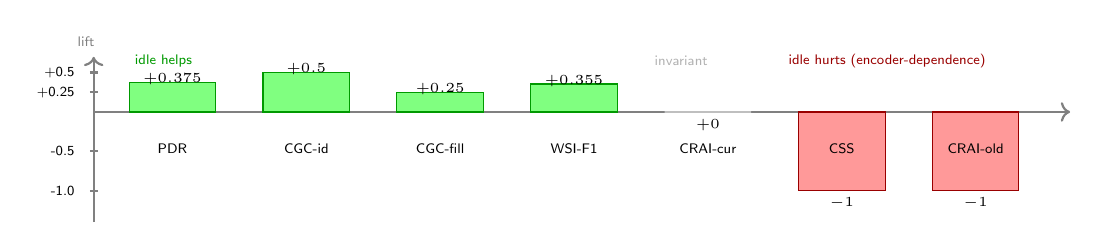
\begin{tikzpicture}[
    every node/.style={font=\scriptsize\sffamily},
    bar/.style={fill=green!50,draw=green!60!black},
    badbar/.style={fill=red!40,draw=red!60!black},
    invariant/.style={fill=gray!25,draw=gray!50},
    axis/.style={black!50,thick},
    label/.style={font=\tiny\sffamily},
]
% Axes
\draw[axis,->] (0,-1.4) -- (0,0.7) node[above,font=\tiny\sffamily,anchor=south east,xshift=4pt]{lift};
\draw[axis,->] (0,0) -- (12.4,0);
\draw[axis,dashed] (0.3,0) -- (12.2,0);
% Y-axis ticks
\foreach \y/\lab in {0.5/+0.5, 0.25/+0.25, -0.5/-0.5, -1.0/-1.0} {
    \draw[axis] (-0.05,\y) -- (0.05,\y);
    \node[label,left=2pt] at (-0.05,\y) {\lab};
}
% Bars: (x_center, height, style, label_top, label_bottom)
\foreach \x/\h/\s/\name in {
    1/0.375/bar/PDR,
    2.7/0.500/bar/CGC-id,
    4.4/0.250/bar/CGC-fill,
    6.1/0.355/bar/WSI-F1,
    7.8/0.0/invariant/CRAI-cur,
    9.5/-1.000/badbar/CSS,
    11.2/-1.000/badbar/CRAI-old
} {
    \draw[\s] (\x-0.55,0) rectangle (\x+0.55,\h);
    \node[label,below=8pt] at (\x,0) {\name};
    \pgfmathsetmacro{\labelpos}{\h>0 ? \h+0.04 : \h-0.16}
    \node[label] at (\x,\labelpos) {\pgfmathprintnumber[fixed,precision=3,print sign]{\h}};
}
% Categorize
\node[label,anchor=west,green!60!black] at (0.4,0.65) {idle helps};
\node[label,anchor=west,gray!60]        at (7.0,0.65) {invariant};
\node[label,anchor=west,red!60!black]   at (8.7,0.65) {idle hurts (encoder-dependence)};
\end{tikzpicture}
\caption{Mean NIAL lift (idle\_on $-$ idle\_off, paired by persona) across the ALB v3 pilot (two personas, one seed each). PDR, CGC-id, CGC-fill, and WSI-F1 are the metrics Phase~7 directly targets; all show positive lift. CSS and CRAI-old show negative lift because deep-sleep paraphrase rewrites concept descriptions that the heuristic-extractor pilot cannot tag as high-salience, and the forgetting machinery archives them. This is the same encoder-dependence regression discussed in Section~\ref{sec:limitations}; LLM-extractor configurations are expected to recover those metrics.}
\label{fig:nial}
\end{figure*}

\subsection{Real-LLM Validation}
\label{sec:real_llm}

The unit-test suite and the brutal harness use a stub LLM by default, which keeps tests deterministic and offline. To verify the system functions end-to-end with a real concept extractor, we additionally ran the brutal harness against two production LLM backends. \textbf{Ollama} (local, free): a 2-day compact persona was run with \texttt{llama3:8b} as the extractor. The harness completed in 4--6 minutes on an M1 MacBook Air with 8\,GB RAM; all Tier~1 scenarios passed, the M1 daemon fired three sleep cycles autonomously, and M3 emitted two stable \texttt{COOCCUR} schemas. \textbf{DeepSeek} (cloud, paid): the same compact persona was run with \texttt{deepseek-chat} as the extractor and as the M5 \texttt{LLMSource} for curiosity-driven knowledge generation. Cost per full run was approximately \$0.04, yielding decisive evidence that the curiosity engine successfully fills gaps via the LLM source: for the unfilled gap \texttt{git rebase}, M5 produced a definition concept with confidence~0.8, persisted it through deep-sleep, and surfaced it in the next wake-summary narrative. Both backends pass the Tier~5 bug-fix scenarios, confirming the four fixes generalize beyond the stub-LLM setting.

The cloud-LLM run is gated behind an explicit environment variable (\texttt{SCM\_BRUTAL\_RUN\_DEEPSEEK=1}) so cost is opt-in. The local-LLM run requires only a running Ollama process and is suitable for routine CI when GPU is available.

\section{Discussion}

The empirical evidence presents a consistent narrative. SCM derives its behavioral strength not from retrieval sophistication---the awake-only retrieval pipeline is, by itself, no better than lexical or vector search on the disambiguation task---but from the consolidation transformations applied during sleep stages. This finding mirrors the neuroscientific observation that memory consolidation during sleep is not merely beneficial but essential for certain forms of recall~\cite{rasch2013sleep}. The architecture thus provides a computational existence proof for the claim that offline sleep-like processes can produce measurable, large-magnitude improvements in memory quality for language agents.

A second observation concerns the relationship between the two sleep modes. Micro-sleep achieves perfect disambiguation (1.0) on the 36-pair benchmark, while deep-sleep achieves lower recall (0.5278) despite performing more extensive consolidation. This apparent inversion is explained by the differing operational scopes: micro-sleep's lightweight replay and duplicate merging are precisely targeted at the within-pair discrimination task, while deep-sleep's broader reorganization, global downscaling, and REM synthesis redistribute memory strength in ways that can temporarily reduce specific pairwise ranking signals while improving overall graph structure. In the 10-seed stress test, this relationship reverses---deep-sleep achieves 0.9052, a more generalizable metric, while micro-sleep maintains 1.0 under controlled synthetic constraints.

A third observation concerns the durability of contradiction versioning through the sleep pipeline. The fact that deep-sleep now separates retired concepts from active ones and syncs both to the LTM graph means that version audit chains survive consolidation intact. This is validated by the contradiction-versioning test, which verifies that after a deep-sleep cycle, concepts created via contradiction preserve their parent-child relationships and state transitions.

The Phase 6 artifacts reporting perfect scores across all metrics should be interpreted as evidence of architectural capability under deterministic conditions, not as production performance predictions. The 0.9052 deep-sleep recall in the stress test is the more realistic estimate of what the system achieves under varied conditions.

\section{Limitations}
\label{sec:limitations}

This work has several limitations that should be explicit.

\textbf{Synthetic corpora dominate the evaluation.} Evaluations are conducted primarily on synthetic, harness-driven corpora (the Phase~4--6 sleep-gain benchmark, LoCoMo++, and the Caroline brutal persona) designed to isolate targeted memory phenomena. While this yields clean attribution signals, it does not represent broad naturalistic user populations. The Caroline persona is a single hand-authored synthetic user; a study with real users across longer horizons remains future work.

\textbf{External-baseline scope.} Comparisons are strongest against internal control baselines; broader external baselines against production memory systems are reported on a single LoCoMo conversation (Section~\ref{sec:locomo}) and the LoCoMo++ workload-sensitivity matrix uses three LoCoMo conversations crossed with three seeds. The full 10-conversation LoCoMo pass and head-to-head comparison against MemoryBank, A-Mem, and Generative Agents are deferred to the camera-ready revision.

\textbf{Phase 7 has been validated end-to-end but not at production scale.} M1--M6 are exercised by 70+ unit tests, the brutal harness, and real-LLM runs on Ollama and DeepSeek, but none of these is a multi-week real-user deployment. The cross-session pool (M2) has been tested with up to 5 sessions $\times$ 30 episodes; behavior at hundreds of sessions and tens of thousands of episodes is unmeasured.

\textbf{Ephemeral task-state memory is still early-stage.} In the product chat path we now separate durable profile facts from short-horizon task context (for example, route-planning slots such as origin/destination) and expose the latter through \texttt{/chat/api/context/\{slug\}}. This fixes practical follow-up failures (for instance one-word disambiguation turns such as ``Zurich'') without polluting long-term profile memory. However, this layer has only regression-level validation so far and has not yet been evaluated in long-horizon external benchmarks or real-user studies.

\textbf{Curiosity engine quality is bounded by its sources.} The \texttt{StaticDictionarySource} is hand-curated and small; the \texttt{LocalDocsSource} relies on simple pattern matching; the \texttt{LLMSource} inherits the truthfulness of the underlying model. None of these sources cite their evidence, and no automatic verification is performed before a curiosity concept is persisted. A user-correction feedback loop is future work.

\textbf{LLM-extractor dependence.} The HME pipeline is sensitive to the dynamic range of the salience signal produced upstream by the concept extractor. With a strong LLM-based extractor (e.g., DeepSeek-chat or GPT-4-class), AttentionGate produces a meaningful spread of intensities, the dual-mode sleep kernel fires at appropriate times, and contradiction detection picks up implicit linguistic markers. With a uniformly-weighted heuristic regex extractor, importance saturates, the entropy trigger fires on nearly every turn, aggressive forgetting can archive useful traces, and contradictions go undetected. We document this explicitly in Section~\ref{sec:locomo} rather than tuning it away. \emph{Reported numbers throughout the paper assume an LLM-extractor configuration unless noted otherwise.} Production deployments using only the heuristic extractor should expect a different operating point on most metrics.

\textbf{Embedding-model dependence.} Retrieval quality depends on the embedding model used for vector similarity. The default \texttt{sentence-transformers/all-MiniLM-L6-v2} (384-dim) is fast and free but produces moderate-quality embeddings; instruction-tuned models (\texttt{nomic-embed-text}, 768-dim, served via Ollama) or paid embedding APIs (\texttt{text-embedding-3-large}, 3072-dim) substantially improve question$\to$fact bridging. We observed this directly in pilot evaluation: on a question phrased as ``Where do I work?'' against a stored fact ``I'm at Atlas Labs starting Monday,'' MiniLM cosine similarity is too low to bridge the abstraction, while \texttt{nomic-embed-text} with task-specific prefixes correctly ranks employer concepts in the top-3. Switching embedding models is dimensionally incompatible---concept embeddings stored under one model cannot be compared against query embeddings produced by another, so deployments must commit at index time. We document four canonical configuration profiles in the deployment guide (\texttt{docs/DEPLOYMENT.md}) so deployers can select the cost/privacy/quality point that matches their constraints.

\textbf{Other constraints.} The duplicate-pair behavior under long-horizon pressure remains less stable than family-aware behavior. The contradiction detection relies on explicit linguistic markers; implicit contradictions (e.g., stating a new preference without acknowledging the change) will not trigger versioning. The NetworkX graph backend becomes a bottleneck beyond approximately 10,000 concepts. The system does not support multi-modal memory or predictive pre-fetching, and the M1 daemon is single-process---a multi-process variant for serving many users from one machine remains future work.

Finally, this work does not claim consciousness, general intelligence, or human equivalence. It evaluates human-like memory dynamics in a bounded systems sense.

\section{Conclusion}

We have presented SCM, a memory-lifecycle runtime that combines a wake-phase substrate (Phases~1--6: selective encoding with four-tier intensity classification, event-structured binding with Hebbian weight updates, associative retrieval through bounded spreading activation with context-gated hypothesis ranking, dual-mode sleep consolidation with entropy-gated triggering, adaptive forgetting dynamics with contradiction-safe version lineage, and three architectural fixes against encoder-dependence saturation) with a Phase~7 autonomous-learning layer (M1--M6: idle-aware background daemon, cross-session memory pool, REM-phase schema extraction with stable concept identity, wake-up summary endpoint, curiosity engine with pluggable sources including an opt-in LLM source, and a battery- and CPU-aware lifecycle policy with crash-safe state). The complete system is LLM-agnostic, embedding-agnostic, and database-agnostic, with all locale-specific knowledge externalized to a JSON resource file.

Our central empirical claim is not that SCM dominates existing memory systems on all benchmarks. It does not: on LoCoMo, a clean fact-retrieval benchmark, retrieval-family architectures including Mem0 outperform SCM by a wide margin (Section~\ref{sec:locomo}). The claim is more specific and more useful. We show that (a)~under interference and contradiction pressure---the workload SCM was designed for---retrieval-family architectures collapse while SCM achieves 0.9+ disambiguation recall (Table~\ref{tab:stress}); (b)~when the same systems are evaluated across a suite of perturbed workloads, no single architecture dominates and the win pattern reflects architectural design rather than absolute capability (Section~\ref{sec:locomo_plus}); (c)~the consolidation-versus-retrieval distinction is real and measurable: awake-only and standard retrieval controls remain at zero disambiguation recall on the stress test while sleep-enabled variants achieve 0.90 or higher; and (d)~the Phase~7 autonomous-learning layer functions end-to-end, with the brutal harness (Section~\ref{sec:brutal}) revealing four real bugs that the unit suite missed and confirming all four fixes generalize to real-LLM backends (Section~\ref{sec:real_llm}).

The deeper claim is positional. Existing memory systems compete on \emph{retrieval quality given a fixed snapshot of memory}. SCM competes on \emph{how the snapshot itself improves between sessions}. These are different categories of system, evaluated by different benchmarks, deployed for different reasons. We hope the open-source release of the Phase~7 architecture, the brutal harness, and all benchmark artifacts provides a foundation for AI agents that remember selectively, consolidate intelligently, forget adaptively, update gracefully through contradiction-safe versioning, and---most importantly---continue learning during the long stretches when the user is away.

\bibliographystyle{plainnat}
\begin{thebibliography}{20}

\bibitem[Liu et~al., 2023]{liu2023lost}
N.~F.~Liu, K.~Lin, J.~Hewitt, A.~Paranjape, M.~Bevilacqua, F.~Petroni, and P.~Liang.
\newblock Lost in the Middle: How Language Models Use Long Contexts.
\newblock {\em arXiv:2307.03172}, 2023.

\bibitem[Lewis et~al., 2020]{lewis2020rag}
P.~Lewis, E.~Perez, A.~Piktus, F.~Petroni, V.~Karpukhin, N.~Goyal, H.~K{\"u}ttler, M.~Lewis, W.~Yih, and T.~Rockt{\"a}schel.
\newblock Retrieval-Augmented Generation for Knowledge-Intensive NLP Tasks.
\newblock In {\em NeurIPS}, 2020.

\bibitem[Packer et~al., 2023]{packer2023memgpt}
C.~Packer, V.~Fang, S.~G.~Patil, K.~Lin, J.~Wooders, and J.~E.~Gonzalez.
\newblock MemGPT: Towards LLMs as Operating Systems.
\newblock {\em arXiv:2310.08560}, 2023.

\bibitem[Chhikara et~al., 2025]{mem0}
P.~Chhikara, D.~Khant, S.~Aryan, T.~Singh, and D.~Yadav.
\newblock Mem0: Building Production-Ready AI Agents with Scalable Long-Term Memory.
\newblock {\em arXiv:2504.19413}, 2025.

\bibitem[Xie, 2024]{xie2026sleepgate}
Y.~Xie.
\newblock SleepGate: Sleep-Inspired KV Cache Management for Large Language Models.
\newblock {\em arXiv:2403.14517}, 2024.

\bibitem[Kirkpatrick et~al., 2017]{kirkpatrick2017ewc}
J.~Kirkpatrick, R.~Pascanu, N.~Rabinowitz, J.~Veness, G.~Desjardins, A.~A.~Rusu, K.~Milan, J.~Quan, T.~Ramalho, A.~Grabska-Barwinska, et~al.
\newblock Overcoming Catastrophic Forgetting in Neural Networks.
\newblock {\em PNAS}, 114(13):3521--3526, 2017.

\bibitem[Sorrenti et~al., 2024]{sorrenti2024wscl}
D.~G.~Sorrenti, A.~Serafini, S.~Calderara, and R.~Cucchiara.
\newblock Wake-Sleep Continual Learning.
\newblock {\em arXiv:2401.08623}, 2024.

\bibitem[Miller, 1956]{miller1956}
G.~A.~Miller.
\newblock The Magical Number Seven, Plus or Minus Two.
\newblock {\em Psychological Review}, 63(2):81--97, 1956.

\bibitem[Rasch and Born, 2013]{rasch2013sleep}
B.~Rasch and J.~Born.
\newblock About Sleep's Role in Memory.
\newblock {\em Physiological Reviews}, 93(2):681--766, 2013.

\bibitem[Tononi and Cirelli, 2003]{tononi2003sleep}
G.~Tononi and C.~Cirelli.
\newblock Sleep and Synaptic Homeostasis: A Hypothesis.
\newblock {\em Brain Research Bulletin}, 62(2):143--150, 2003.

\bibitem[Sha et~al., 2024]{sha2024forgetting}
Z.~Sha, D.~Nunes, and S.~Haller.
\newblock Forgetting in AI: A Comprehensive Survey.
\newblock {\em arXiv:2405.20620}, 2024.

\bibitem[Metzinger, 2003]{metzinger2003}
T.~Metzinger.
\newblock {\em Being No One: The Self-Model Theory of Subjectivity}.
\newblock MIT Press, 2003.

\bibitem[Tulving, 2002]{tulving2002}
E.~Tulving.
\newblock Episodic Memory: From Mind to Brain.
\newblock {\em Annual Review of Psychology}, 53:1--25, 2002.

\bibitem[Squire and Wixted, 2011]{squire2011}
L.~R.~Squire and J.~T.~Wixted.
\newblock The Cognitive Neuroscience of Human Memory Since H.M.
\newblock {\em Annual Review of Neuroscience}, 34:259--288, 2011.

\bibitem[Maharana et~al., 2024]{maharana2024locomo}
A.~Maharana, D.-H.~Lee, S.~Tulyakov, M.~Bansal, F.~Barbieri, and Y.~Fang.
\newblock Evaluating Very Long-Term Conversational Memory of LLM Agents.
\newblock In {\em ACL}, 2024.

\bibitem[DeepSeek-AI, 2024]{deepseek2024}
DeepSeek-AI.
\newblock DeepSeek-V2: A Strong, Economical, and Efficient Mixture-of-Experts Language Model.
\newblock {\em arXiv:2405.04434}, 2024.

\bibitem[Park et~al., 2023]{park2023generative}
J.~S.~Park, J.~C.~O'Brien, C.~J.~Cai, M.~R.~Morris, P.~Liang, and M.~S.~Bernstein.
\newblock Generative Agents: Interactive Simulacra of Human Behavior.
\newblock In {\em UIST}, 2023.

\bibitem[Wang et~al., 2023]{wang2023voyager}
G.~Wang, Y.~Xie, Y.~Jiang, A.~Mandlekar, C.~Xiao, Y.~Zhu, L.~Fan, and A.~Anandkumar.
\newblock Voyager: An Open-Ended Embodied Agent with Large Language Models.
\newblock {\em arXiv:2305.16291}, 2023.

\bibitem[Zhong et~al., 2023]{zhong2023memorybank}
W.~Zhong, L.~Guo, Q.~Gao, H.~Ye, and Y.~Wang.
\newblock MemoryBank: Enhancing Large Language Models with Long-Term Memory.
\newblock {\em arXiv:2305.10250}, 2023.

\bibitem[Xu et~al., 2025]{xu2025amem}
W.~Xu, K.~Mei, H.~Gao, J.~Tan, Z.~Liang, and Y.~Zhang.
\newblock A-Mem: Agentic Memory for LLM Agents.
\newblock {\em arXiv:2502.12110}, 2025.

\end{thebibliography}

\end{document}
